\documentclass[12pt]{article}
\usepackage[english]{babel}
\usepackage{lipsum}
\usepackage[square, numbers]{natbib}
\bibliographystyle{plainurl}
\usepackage{url}
\usepackage[utf8x]{inputenc}
\usepackage{amsmath}
\usepackage{mathtools}
\usepackage{mathtools,siunitx}
\sisetup{detect-all}
\usepackage{graphicx}
\graphicspath{{images/}}
\usepackage{parskip}
\usepackage{fancyhdr}
\usepackage{vmargin}
\usepackage{hyperref}
\usepackage{todonotes}
\usepackage{textcomp}
\usepackage{float}
\usepackage{listings}
\usepackage{enumitem}
\usepackage{caption}
\usepackage{listings}
\usepackage{cleveref}


\usepackage{color} %red, green, blue, yellow, cyan, magenta, black, white
\definecolor{mygreen}{RGB}{28,172,0} % color values Red, Green, Blue
\definecolor{mylilas}{RGB}{170,55,241}
\setmarginsrb{2 cm}{2.5 cm}{2 cm}{2.5 cm}{1 cm}{1 cm}{1 cm}{1 cm}
\presetkeys{todonotes}{fancyline}{}



%%%%%%%%%%%%%%%%%%%%%%%%%% TITLE %%%%%%%%%%%%%%%%%%%
\title{Infrastructure Development in Dubai}
\author{A. Scharf}	
\date{\today}

\makeatletter
\let\thetitle\@title
\let\theauthor\@author
\let\thedate\@date

\providecommand\add@text{}
\newcommand\tagaddtext[1]{%
  \gdef\add@text{#1\gdef\add@text{}}}% 
\renewcommand\tagform@[1]{%
  \maketag@@@{\llap{\add@text\quad}(\ignorespaces#1\unskip\@@italiccorr)}%
}
\makeatother

\pagestyle{fancy}
\fancyhf{}
\rhead{\theauthor}
\lhead{\thetitle}
\cfoot{\thepage}

%% Uncomment the following line if subsections shall be numbered with alphabetic characters instead of numbers!
%\renewcommand{\thesubsection}{\thesection.\alph{subsection}}



\begin{document}

\lstset{language=Matlab,%
    %basicstyle=\color{red},
    breaklines=true,%
    morekeywords={matlab2tikz},
    keywordstyle=\color{blue},%
    morekeywords=[2]{1}, keywordstyle=[2]{\color{black}},
    identifierstyle=\color{black},%
    stringstyle=\color{mylilas},
    commentstyle=\color{mygreen},%
    showstringspaces=false,%without this there will be a symbol in the places where there is a space
    numbers=left,%
    numberstyle={\tiny \color{black}},% size of the numbers
    numbersep=9pt, % this defines how far the numbers are from the text
    emph=[1]{for,end,break},emphstyle=[1]\color{red}, %some words to emphasise
    %emph=[2]{word1,word2}, emphstyle=[2]{style},
}

%%%%%%%%%%%%%%%%%%%% Titlepage start %%%%%%%%%%%%%%%%%%%%%%%%%%%%

\begin{titlepage}
	\centering
    \vspace*{0.5 cm}
    
\includegraphics[scale = 0.15]{images/upslogo}\\[1.0 cm]

	\textsc{\Large M2 - TSI}\\[0.5 cm]

	\textsc{\large UE52 Earth Observation Report}\\[0.5 cm]	
	\vspace{1cm}
	\rule{\linewidth}{0.2 mm} \\[0.4 cm]
	{ \huge \bfseries \thetitle}\\
	\rule{\linewidth}{0.2 mm}
	\\[0.5cm]
		\textsc{}
		\\[2.5 cm]

	\vspace{1cm}
	\emph{Author:}\\
	Arthur Scharf
	\vspace{2cm}
	
	{\large \today }\\[2 cm]
 
	\vfill
	
\end{titlepage}
%%%%%%%%%%%%%%%%%%% Titlepage end %%%%%%%%%%%%%%%%%%%%%%%%%%%%%%%


%%%%%%%%%%%%%%%%% include content %%%%%%%%%%%%%
\section{Introduction}
Dubai is a city located in the United Arab Emirates near the Persian Gulf and is well known and acknowledged as a global city. Since oil was discovered in the late 1906's, Dubai started to expand very fast. However, nowadays only about 5\% of Dubai's revenue is connected to the black gold, but instead Dubai is known for financial services, tourism and aviation \citep{wiki:dubai}. Also, Dubai is known for having the world's tallest building, the Burj Khalifa and its extremely high living expenses. This leads to the question how, and in which way, Dubai has been expanding and growing since the late 1960's.

In this study the development of Dubai's infrastructure will analysed by using satellite images within the visible bands / spectrum.
Since analysing infrastructure from space in the visible spectrum is a difficult topic, this report will focus on two different methods: first, an analysis of the captured colours, i.e. water and land, by using supervised classification (kNN algorithm) and second, a pattern and structure analysis using edge detection techniques and morphological filtering.

To be able to analyse the actual development of structure, land and water evolution LandSat Data from since 1984 until 2016 will be used - one satellite image per year within the same or a close month, depending  on the cloud conditions.

In particular, the following sections will cover the involved satellites and its instruments that are used to capture the images. Also, the images itself will be looked closer at, especially regarding resolution, image period etc. After, the aforementioned methods and the overall analysis approach will be explained in more detail. The results of this analysis will then  be discussed and a conclusion given, stating the findings and a future outlook on this particular topic of infrastructure development observation.

\section{Satellite Instruments}
Since this report covers a period of about 32 years, satellite imaginary from different satellite platforms will be used. To ensure a minimum compatibility between the images, e.g. regarding resolution etc., images from the same satellite family will be used - in particular LandSat satellites 4, 5, 7 and 8.
The LandSat project is a joint program of the U.S. Geological Survey and (USGS) and NASA, with the first satellite launch in 1972 \citep{pub:usgs}, to provide continuous global earth observation data coverage .

Even though the resolution is only moderate, the LandSat satellites provide a continuous and global coverage - resulting in a vast amount of image data that reaches back around 4 decades. The data is made publicly available for free within the Landsat remote sensing (LRS) component of USGS in the EROS data centre.\citep{remote:usgs}

A first initial screening of the image data that is available from LandSat-1 to LandSat-3 revealed very quickly that those image data might not be very suitable for a proper analysis, since the very early LandSat satellites used Taperecorders to actually record images, so the retrieved resolution and image quality is not very much comparable to the later LandSat versions. Thus, LandSat-1 to LandSat-3 data is not used in the Analysis.

Also, for the purpose of this study, only the visible spectral bands are used in the image data. However, for the sake of completeness, the following subsections give an overview of all available spectral bands in the respective instruments.

\subsection{LandSat-4 and 5 Thematic Mapper}
LandSat-4 was a project by NASA, NOAA, EOSAT and USGS and was launched on 16th July 1982 on a Delta 3920 rocket. The satellite weighted about 1942kg and used a Hydrazine propulsion system for its attitude control system. The Communication System used S, X, L and  Ku bands and had a data rate of about 85 Mbps on the downlink via the Tracking and Data Relay Satellite System (TDRSS). The satellite was launched in a sun-synchronous circular orbit with an inclination of 98.2° at a height of 705km \citep{l4:usgs}.

%\footnote{https://landsat.usgs.gov/landsat-4-history}

LandSat-4 and 5 were two identical satellites, with LandSat-5 being a backup satellite that outlived LandSat-4 and provided data until 2013 \citep{l5:wiki,l5:usgs}.
%\todo{en.wikipedia.org/wiki/Landsat_4 landsat.usgs.gov/landsat-5-history}

Both satellites carried two observation instruments, the Multispectral Scanner (MSS) and the Thematic Mapper (TM) with the following available spectral bands:

\begin{table} [h!]
	\centering
	\begin{tabular}{ | c | c | c | c |}
	\hline
	\textbf{No.} & \textbf{Band} & \textbf{$\lambda$} & \textbf{resolution} \\
	\hline
	Band 4 & Visible & 0.5 - 0.6 $\mu m$ & {57 x 79 m} \\
	Band 5 & Visible & 0.6 - 0.7 $\mu m$ & {57 x 79 m} \\
	Band 6 & Near IR & 0.7 - 0.8 $\mu m$ & {57 x 79 m} \\
	Band 7 & Near IR & 0.8 - 1.1 $\mu m$ & {57 x 79 m} \\
	\hline
	\end{tabular}
	\caption{MSS Instrument on Landsat 4 and 5\citep{l4:usgs}\citep{l5:usgs}}
	\label{tab:L45MSS}
\end{table}

\begin{table}[h!]
	\centering
	\begin{tabular}{ | c | c | c | c |}
	\hline
	\textbf{No.} & \textbf{Band} & \textbf{$\lambda$} & \textbf{resolution} \\
	\hline
	Band 1 & Visible & 0.45 - 0.52 $\mu m$ & {30 m} \\
	Band 2 & Visible & 0.52 - 0.60 $\mu m$ & {30 m} \\
	Band 3 & Visible & 0.63 - 0.69 $\mu m$ & {30 m} \\
	Band 4 & Near IR & 0.76 - 0.90 $\mu m$ & {30 m} \\
	Band 5 & Near IR & 1.55 - 1.75 $\mu m$ & {30 m} \\
	Band 6 & Thermal & 10.40 - 12.50 $\mu m$ & {30 m} \\
	Band 7 & Mid IR & 2.08 - 2.35 $\mu m$ & {30 m} \\
	\hline
	\end{tabular}
	\caption{TM Instrument on Landsat 4 and 5\citep{l4:usgs,l5:usgs}}
	\label{tab:L45TM}
\end{table}




\subsection{LandSat-7 Enhanced Thematic Mapper Plus}
LandSat-7, a successor to LandSat-4 and 5 since the launcher during the LandSat-6 launch failed, was launched on 15th April 1999 on a Delta II rocket. This satellite was heavier than its predecessors with about 2200kg and used a more sophisticated downlink method (Solid State Recorders or SSR's) to provide an improved downlink speed of 150Mbps.\\
The satellite was launched the same sun-synchronous circular orbit as LandSat-4 with an inclination of 98.2° at a height of 705km, but with about 15 minutes behind LandSat-4 \citep{l7:usgs}.

Another improvement was done on the Thematic Mapper, here called the Enhanced Thematic Mapper Plus (ETM+), with an increased amount of spectral bands and a panchromatic band with double the resolution compared to the other ones. \Cref{tab:L7ETM} shows a quick overview over the available spectral bands.

\begin{table}[h!]
	\centering
	\begin{tabular}{ | c | c | c | c |}
	\hline
	\textbf{No.} & \textbf{Band} & \textbf{$\lambda$} & \textbf{resolution} \\
	\hline
	Band 1 & Visible & 0.45 - 0.52 $\mu m$ & {30 m} \\
	Band 2 & Visible & 0.52 - 0.60 $\mu m$ & {30 m} \\
	Band 3 & Visible & 0.63 - 0.69 $\mu m$ & {30 m} \\
	Band 4 & Near IR & 0.76 - 0.90 $\mu m$ & {30 m} \\
	Band 5 & Near IR & 1.55 - 1.75 $\mu m$ & {30 m} \\
	Band 6 & Thermal & 10.40 - 12.50 $\mu m$ & {60 m Low \& High Gain} \\
	Band 7 & Mid IR & 2.08 - 2.35 $\mu m$ & {30 m} \\
	Band 8 & Panchromatic & 0.52 - 0.90 $\mu m$ & {15 m} \\
	\hline
	\end{tabular}
	\caption{ETM+ Instrument on Landsat 7\citep{l7:usgs}}
	\label{tab:L7ETM}
\end{table}


\subsection{LandSat-8 Operational Land Imager}
LandSat-8 was another iteration of the LandSat family and was launched on February 11, 2013 on an Atlas-V rocket. Again, this satellite was heaver compared to its predecessors with a weight of 2623kg. Contrary to LandSat-7, two distinct imaging instruments were used, the Operational Land Imager (OLI) and the Thermal Infrared Sensor (TIRS), where the OLI instruments was essentially the ETM+ with an additional detector to observe Cirrus clouds \citep{l7:usgs}. The \cref{tab:L8OLI,tab:L8TIRS} show the appropriate spectral band properties for both instruments.

\begin{table}[h!]
	\centering
	\begin{tabular}{ | c | c | c | c |}
	\hline
	\textbf{No.} & \textbf{Band} & \textbf{$\lambda$} & \textbf{resolution} \\
	\hline
	Band 1 & Visible & 0.43 - 0.45 $\mu m$ & {30 m} \\
	Band 2 & Visible & 0.45 - 0.51 $\mu m$ & {30 m} \\
	Band 3 & Visible & 0.53 - 0.59 $\mu m$ & {30 m} \\
	Band 4 & Red & 0.64 - 0.67 $\mu m$ & {30 m} \\
	Band 5 & Near IR & 0.85 - 0.88 $\mu m$ & {30 m} \\
	Band 6 & SWIR 1 & 1.57 - 1.65  $\mu m$ & {30 m} \\
	Band 7 & SWIR 2 & 2.11 - 2.29 $\mu m$ & {30 m} \\
	Band 8 & Panchromatic & 0.52 - 0.90 $\mu m$ & {15 m} \\
	Band 8 & Cirrus & 1.36 - 1.38 $\mu m$ & {30 m} \\
	\hline
	\end{tabular}
	\caption{OLI Instrument on Landsat 8 \citep{l8:usgs}}
	\label{tab:L8OLI}
\end{table}

\begin{table}[h!]
	\centering
	\begin{tabular}{ | c | c | c | c |}
	\hline
	\textbf{No.} & \textbf{Band} & \textbf{$\lambda$} & \textbf{resolution} \\
	\hline
	Band 10 & TIRS 1 & 10.6 - 11.19 $\mu m$ & {100 m} \\
	Band 11 & TIRS 2 & 11.5 - 12.51 $\mu m$ & {100 m} \\
	\hline
	\end{tabular}
	\caption{TIRS Instrument on Landsat 8 \citep{l8:usgs}}
	\label{tab:L8TIRS}
\end{table}


\section{Satellite Imaginary and Observations}
As explained in the previous chapter, imagery provided by different satellites and satellite instruments were used in this report. This chapter will give a short overview on the used image and their properties. All Images were selected and downloaded via the \textit{EarthExplorer}, a tool provided by the USGS to select earth observation data based on different criteria, such as coordinates (Degree/Minute/Second or WRS-2\footnote{World-Reference-System-2 for LandSat satellites consisting of two numbers, the Path and the Row of the satellite ground track}), different features in the images and data ranges.\\
Also, different data sets provided by different programmes and satellites can be searched \citep{earthexpl}.\\

\subsection{LandSat-4 TM Imagery}

\begin{table} [h!]
	\centering
	\begin{tabular}{| c | c | c | c | c |}
	\hline
	\textbf{Image Number} & \textbf{Resolution} & \textbf{Band} & \textbf{Capture Year} & \textbf{Location} \\ \hline
	LT41600431988027XXX03.jpg & 30 m / pixel& Visible & 1988 & 160/043 (WRS-2) \\ \hline 
	LT41600431990240XXX03.jpg & 30 m / pixel& Visible & 1990 & 160/043 (WRS-2) \\ \hline 
	LT41600431992166XXX02.jpg & 30 m / pixel& Visible & 1992 & 160/043 (WRS-2) \\ \hline 
	\end{tabular}
\end{table}

\subsection{LandSat-5 TM Imagery}
\begin{table}[h!]
	\centering
	\begin{tabular}{| c | c | c | c | c |}
	\hline
	\textbf{Image Number} & \textbf{Resolution} & \textbf{Band} & \textbf{Capture Year} & \textbf{Location} \\ \hline
	LT51600431984136XXX12.jpg & 30 m / pixel& Visible & 1984 & 160/043 (WRS-2) \\ \hline 
	LT51600431985042AAA04.jpg & 30 m / pixel& Visible & 1985 & 160/043 (WRS-2) \\ \hline 
	LT51600431986045XXX05.jpg & 30 m / pixel& Visible & 1986 & 160/043 (WRS-2) \\ \hline 
	LT51600431987272XXX10.jpg & 30 m / pixel& Visible & 1987 & 160/043 (WRS-2) \\ \hline 
	LT51600431989165ISP00.jpg & 30 m / pixel& Visible & 1989 & 160/043 (WRS-2) \\ \hline 
	LT51600431991171ISP00.jpg & 30 m / pixel& Visible & 1991 & 160/043 (WRS-2) \\ \hline 
	LT51600431993160ISP00.jpg & 30 m / pixel& Visible & 1993 & 160/043 (WRS-2) \\ \hline 
	LT51600431994179ISP00.jpg & 30 m / pixel& Visible & 1994 & 160/043 (WRS-2) \\ \hline 
	LT51600431995278ISP00.jpg & 30 m / pixel& Visible & 1995 & 160/043 (WRS-2) \\ \hline 
	LT51600431996345ISP00.jpg & 30 m / pixel& Visible & 1996 & 160/043 (WRS-2) \\ \hline 
	LT51600431997011ISP00.jpg & 30 m / pixel& Visible & 1997 & 160/043 (WRS-2) \\ \hline 
	LT51600431998286XXX01.jpg & 30 m / pixel& Visible & 1998 & 160/043 (WRS-2) \\ \hline 
	LT51600432008138KHC01.jpg & 30 m / pixel& Visible & 2008 & 160/043 (WRS-2) \\ \hline 
	\end{tabular}
\end{table}

For reasons unknown LandSat-5 acquired only very few data during the period of 1998 and 2008 - while researching this interesting data gap it could not be determined if this gap was due to problems or introduced on purpose. However, the MSS, the second instrument on board was powered off in 1999 and then powered back on in 2013, after the TM instrument failed \citep{l5:usgs}.

\subsection{LandSat-7 ETM+ Imagery}

\begin{table} [h!]
	\centering
	\begin{tabular}{| c | c | c | c | c |}
	\hline
	\textbf{Image Number} & \textbf{Resolution} & \textbf{Band} & \textbf{Capture Year} & \textbf{Location} \\ \hline
	LE71600431999265SGS01.jpg & 30 m / pixel& Visible & 1999 & 160/043 (WRS-2) \\ \hline 
	LE71600432000188SGS00.jpg & 30 m / pixel& Visible & 2000 & 160/043 (WRS-2) \\ \hline 
	LE71600432001190EDC00.jpg & 30 m / pixel& Visible & 2001 & 160/043 (WRS-2) \\ \hline 
	LE71600432002273SGS01.jpg & 30 m / pixel& Visible & 2002 & 160/043 (WRS-2) \\ \hline 
	LE71600432003148ASN00.jpg & 30 m / pixel& Visible & 2003 & 160/043 (WRS-2) \\ \hline 
	\end{tabular}
\end{table}

In 2003 the Scan Line Correction (SLC) feature of the ETM+ instrument failed, which led to disturbed images due to the fact that the instrument did not correct the movement of the satellite in orbit while taking images. Due to the heavy image distortion in the area this report is actually focused on (coast of the Emirates, see upper left part of \cref{fig:L7SLCOFF}), this data is discarded for the use within this study, even though image data would be available up until the present day \citep{l7:usgs}.



\begin{figure}[h!]
\centering
\begin{minipage}{.5\textwidth}
	\centering
	\includegraphics[width=\textwidth-3em]{code/imagedata/L7ETM_SLC-off_2003-present/LE71600432010279ASN00}
	\caption{L-7 ETM+ SLC OFF (2010)}
	\label{fig:L7SLCOFF}
\end{minipage}%
\begin{minipage}{.5\textwidth}
	\centering
	\includegraphics[width=\textwidth-3em]{code/imagedata/L7ETM_SLC-on_1999-2003/LE71600432003148ASN00.jpg}
	\caption{L-7 ETM+ SLC ON (2003)}
	\label{fig:L7SLCON}
\end{minipage}
\end{figure}

\subsection{LandSat-8 OLI Imagery}
Since the Images provided by LandSat-7 provided after 2003 were not usable, and LandSat-5 was decommissioned in 2013 \citep{l5:usgs}, the most recent data was selected from LandSat-8. This was done in particular since the resolution and image capture location and orientation is the same as in the previous pictures, even though for this time period newer and high-resolution satellite images would be available. This significantly decreases the effort for the analysis part of this report.

\begin{table} [h!]
	\centering
	\begin{tabular}{| c | c | c | c | c |}
	\hline
	\textbf{Image Number} & \textbf{Resolution} & \textbf{Band} & \textbf{Capture Year} & \textbf{Location} \\ \hline
	LC81600432013151LGN00.jpg & 30 m / pixel& Visible & 2013 & 160/043 (WRS-2) \\ \hline 
	LC81600432014154LGN00.jpg & 30 m / pixel& Visible & 2014 & 160/043 (WRS-2) \\ \hline 
	LC81600432015269LGN00.jpg & 30 m / pixel& Visible & 2015 & 160/043 (WRS-2) \\ \hline 
	LC81600432016352LGN00.jpg & 30 m / pixel& Visible & 2016 & 160/043 (WRS-2) \\ \hline 
	\end{tabular}
\end{table}

\section{Analysis Methods}
After having obtained the relevant images as explained in the previous chapter, the image data had to be processed. For this report in particular, the focus was put on the analysis of the structure that is present in the region of interest (ROI) of the image. Under the assumption that a civilisation that is expanding in an area with enough free space available in the surrounding (as is the case in the quite desert-like area around Dubai), will build houses, roads and other periphery that is required to sustain a civilisation, the hypothesis for image analysis is as follows,\\
\begin{quote}
	\textbf{The more edges and/or junctions are detected the higher the development level of infrastructure.}
\end{quote}

Another assumption that can be made concerning infrastructure development is, that if a city grows, the natural flora and fauna is reduced. This leads to a second hypothesis that can be made.
\begin{quote}
	\textbf{The less water (sea, rivers, lakes) and vegetation is observed the higher the development level of infrastructure.}
\end{quote}

To prove these hypotheses, various methods and techniques have been used, as will be explained in the following sub-chapters.

\subsection{Preprocessing}
\label{subsec:pre}
Since the data gathered from \textit{EarthExplorer} has already been preprocessed, i.e. assembled from different visible spectra, corrected w.r.t. north and watermarked, it needed some initial preprocessing. Also, since the images were not equal in pixel size and did not feature the Region-of-Interest in the same pixel area, a machine-based pre-processing was not feasible in the scope of this project. Thus, all images were edited using a mask of the current borders of Dubai, c.f. \cref{fig:borders}. This was done by masking the borders on the latest 2016-image of LandSat-8, which corresponds the best to the Google-Maps Image (note: \cref{fig:borders} contains Dubai City and Greater Dubai, for the purpose of this report Greater Dubai borders were used). Since, as mentioned, the image sizes did not match and the ROI location varied, the mask was adjusted for every image manually using Photoshop (see e.g. \cref{fig:L8OLI_16}) by overlaying the border mask. As a result each image had a correctly masked Region-of-Interest. An example image is shown in \cref{fig:L8_OLI_16_masked}).
\begin{figure}[h!]
	\centering
	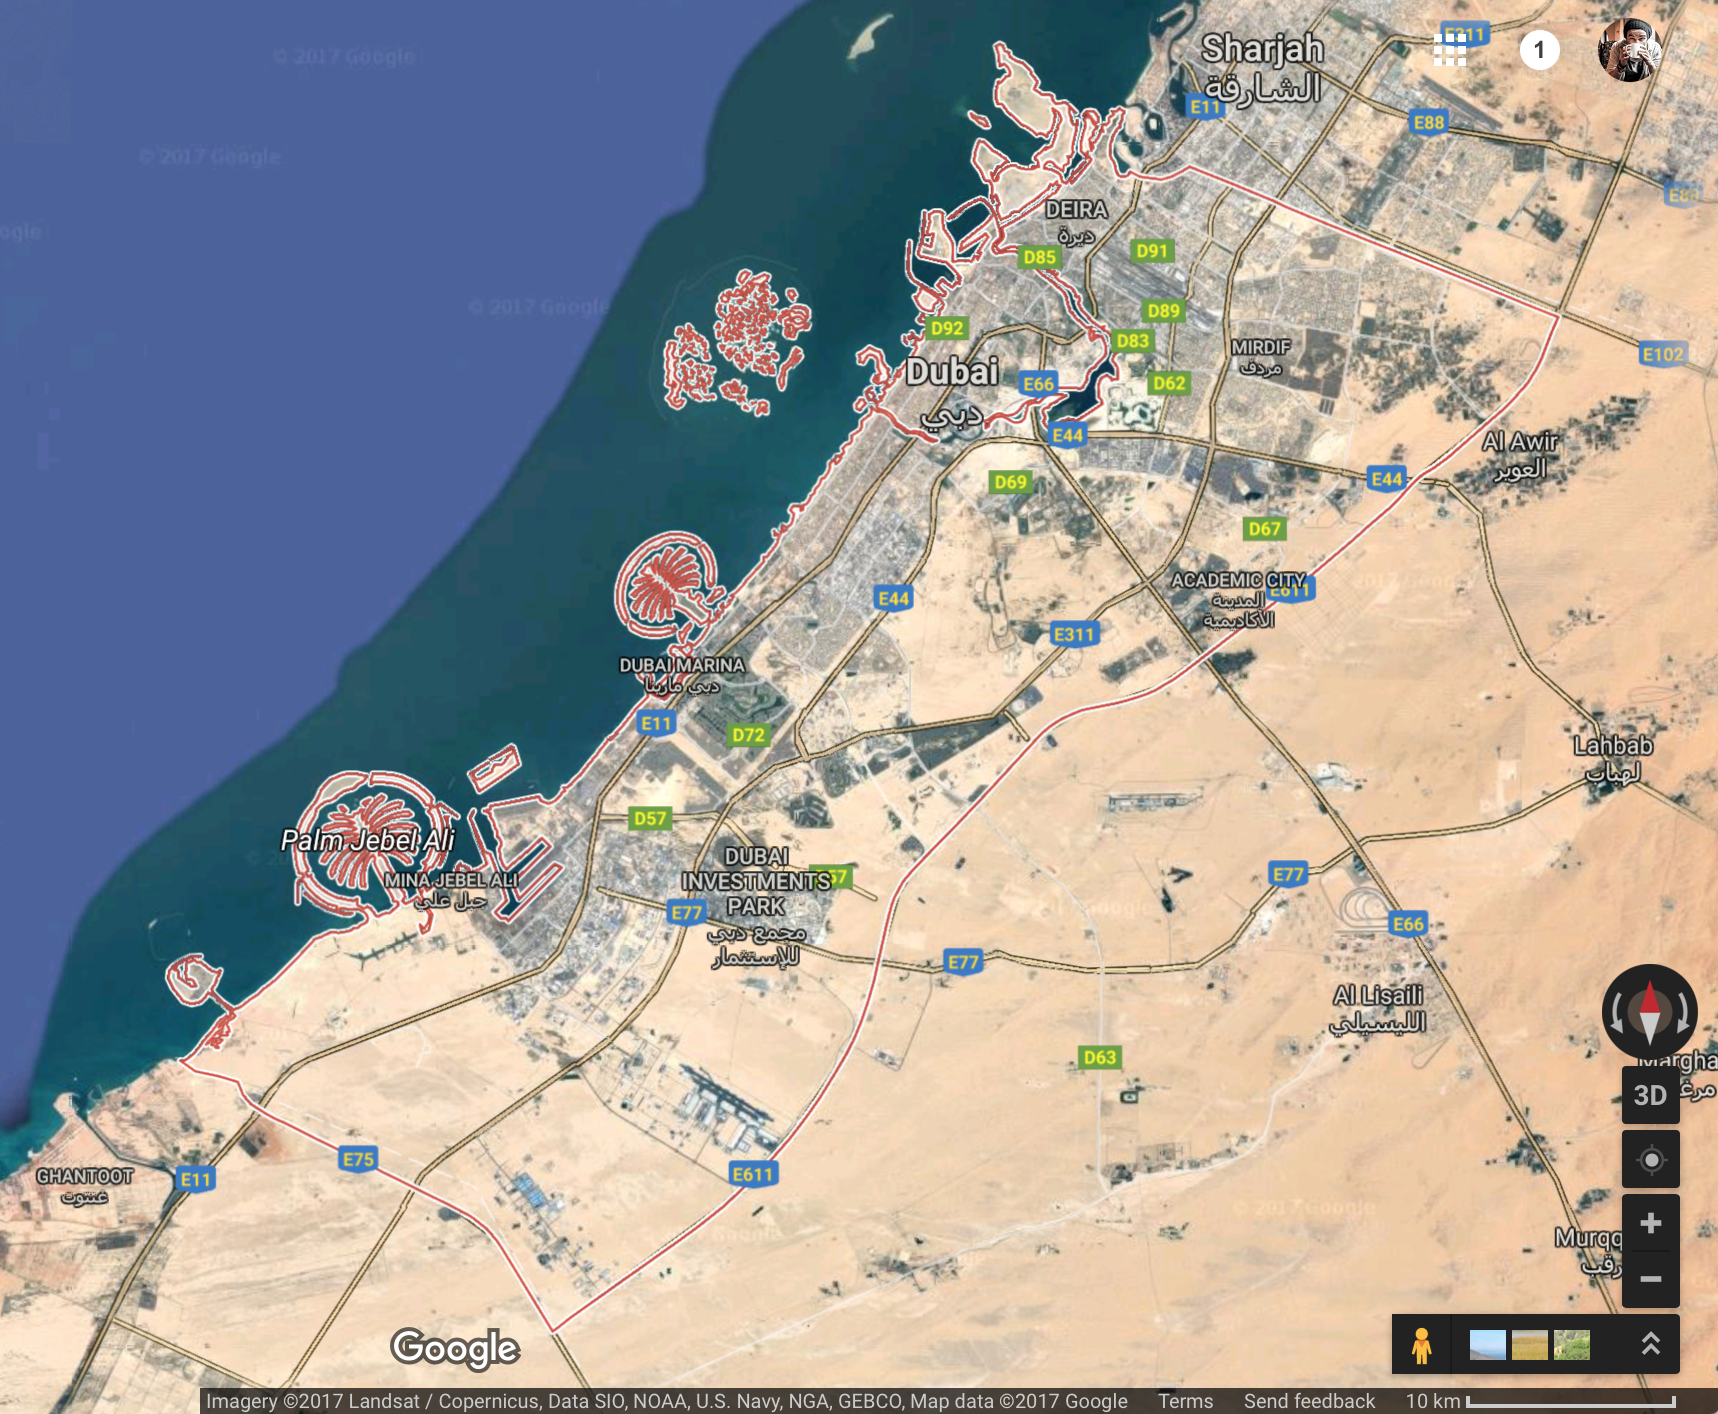
\includegraphics[width=\textwidth]{images/google_dubai.png}
	\caption{Borders of Dubai marked in Red\citep{googlemaps}}
	\label{fig:borders}
\end{figure}
\begin{figure}[h!]
\centering
\begin{minipage}{.5\textwidth}
	\centering
	\includegraphics[width=\textwidth-3em]{code/imagedata/L8OLI_TIRS/LC81600432016352LGN00.jpg}
	\caption{L-8 OLI Image (2016)}
	\label{fig:L8OLI_16}
\end{minipage}%
\begin{minipage}{.5\textwidth}
	\centering
	\includegraphics[width=\textwidth-3em]{code/imagedata/L8OLI_TIRS/LC81600432016352LGN00.png}
	\caption{L-8 OLI Image (2016) masked (ROI)}
	\label{fig:L8_OLI_16_masked}
\end{minipage}
\end{figure}

Having obtained the actual area/region of interest, the image was cropped to include as little overhead pixels as possible to reduce the image size and thus the processing time and effort. Also, cropping the image made it possible to equalise the size of images in terms of pixel width and height. This process is visualised between \cref{fig:L8_OLI_16_masked,fig:L8OLI_16_cropped}. The cropped images were now reduced to a size of 3201x3001 pixels, and the white background was converted to black for easier processing in later stages. \\
During the screening of the images it was also very obvious, that the brightness and colours had significant variation between different pictures. This would vastly affect the analysis w.r.t. to the second hypothesis. This is the reason why the histograms of the images were equalised with the built-in MATLAB function \texttt{imhistmatch} , so that the brightness and colour would match very well in between different images. It was possible to do so, since the images featured the exact same region of interest. The result of this histogram equalisation performed on \cref{fig:L8OLI_16_cropped} can be seen in \cref{fig:L8_OLI_16_equalised}.
The cropping (selecting the ROI) and histogram equalisation was done automatically using Matlab, see \todo{include Matlab code}.


\begin{figure}[h!]
\centering
\begin{minipage}{.5\textwidth}
	\centering
	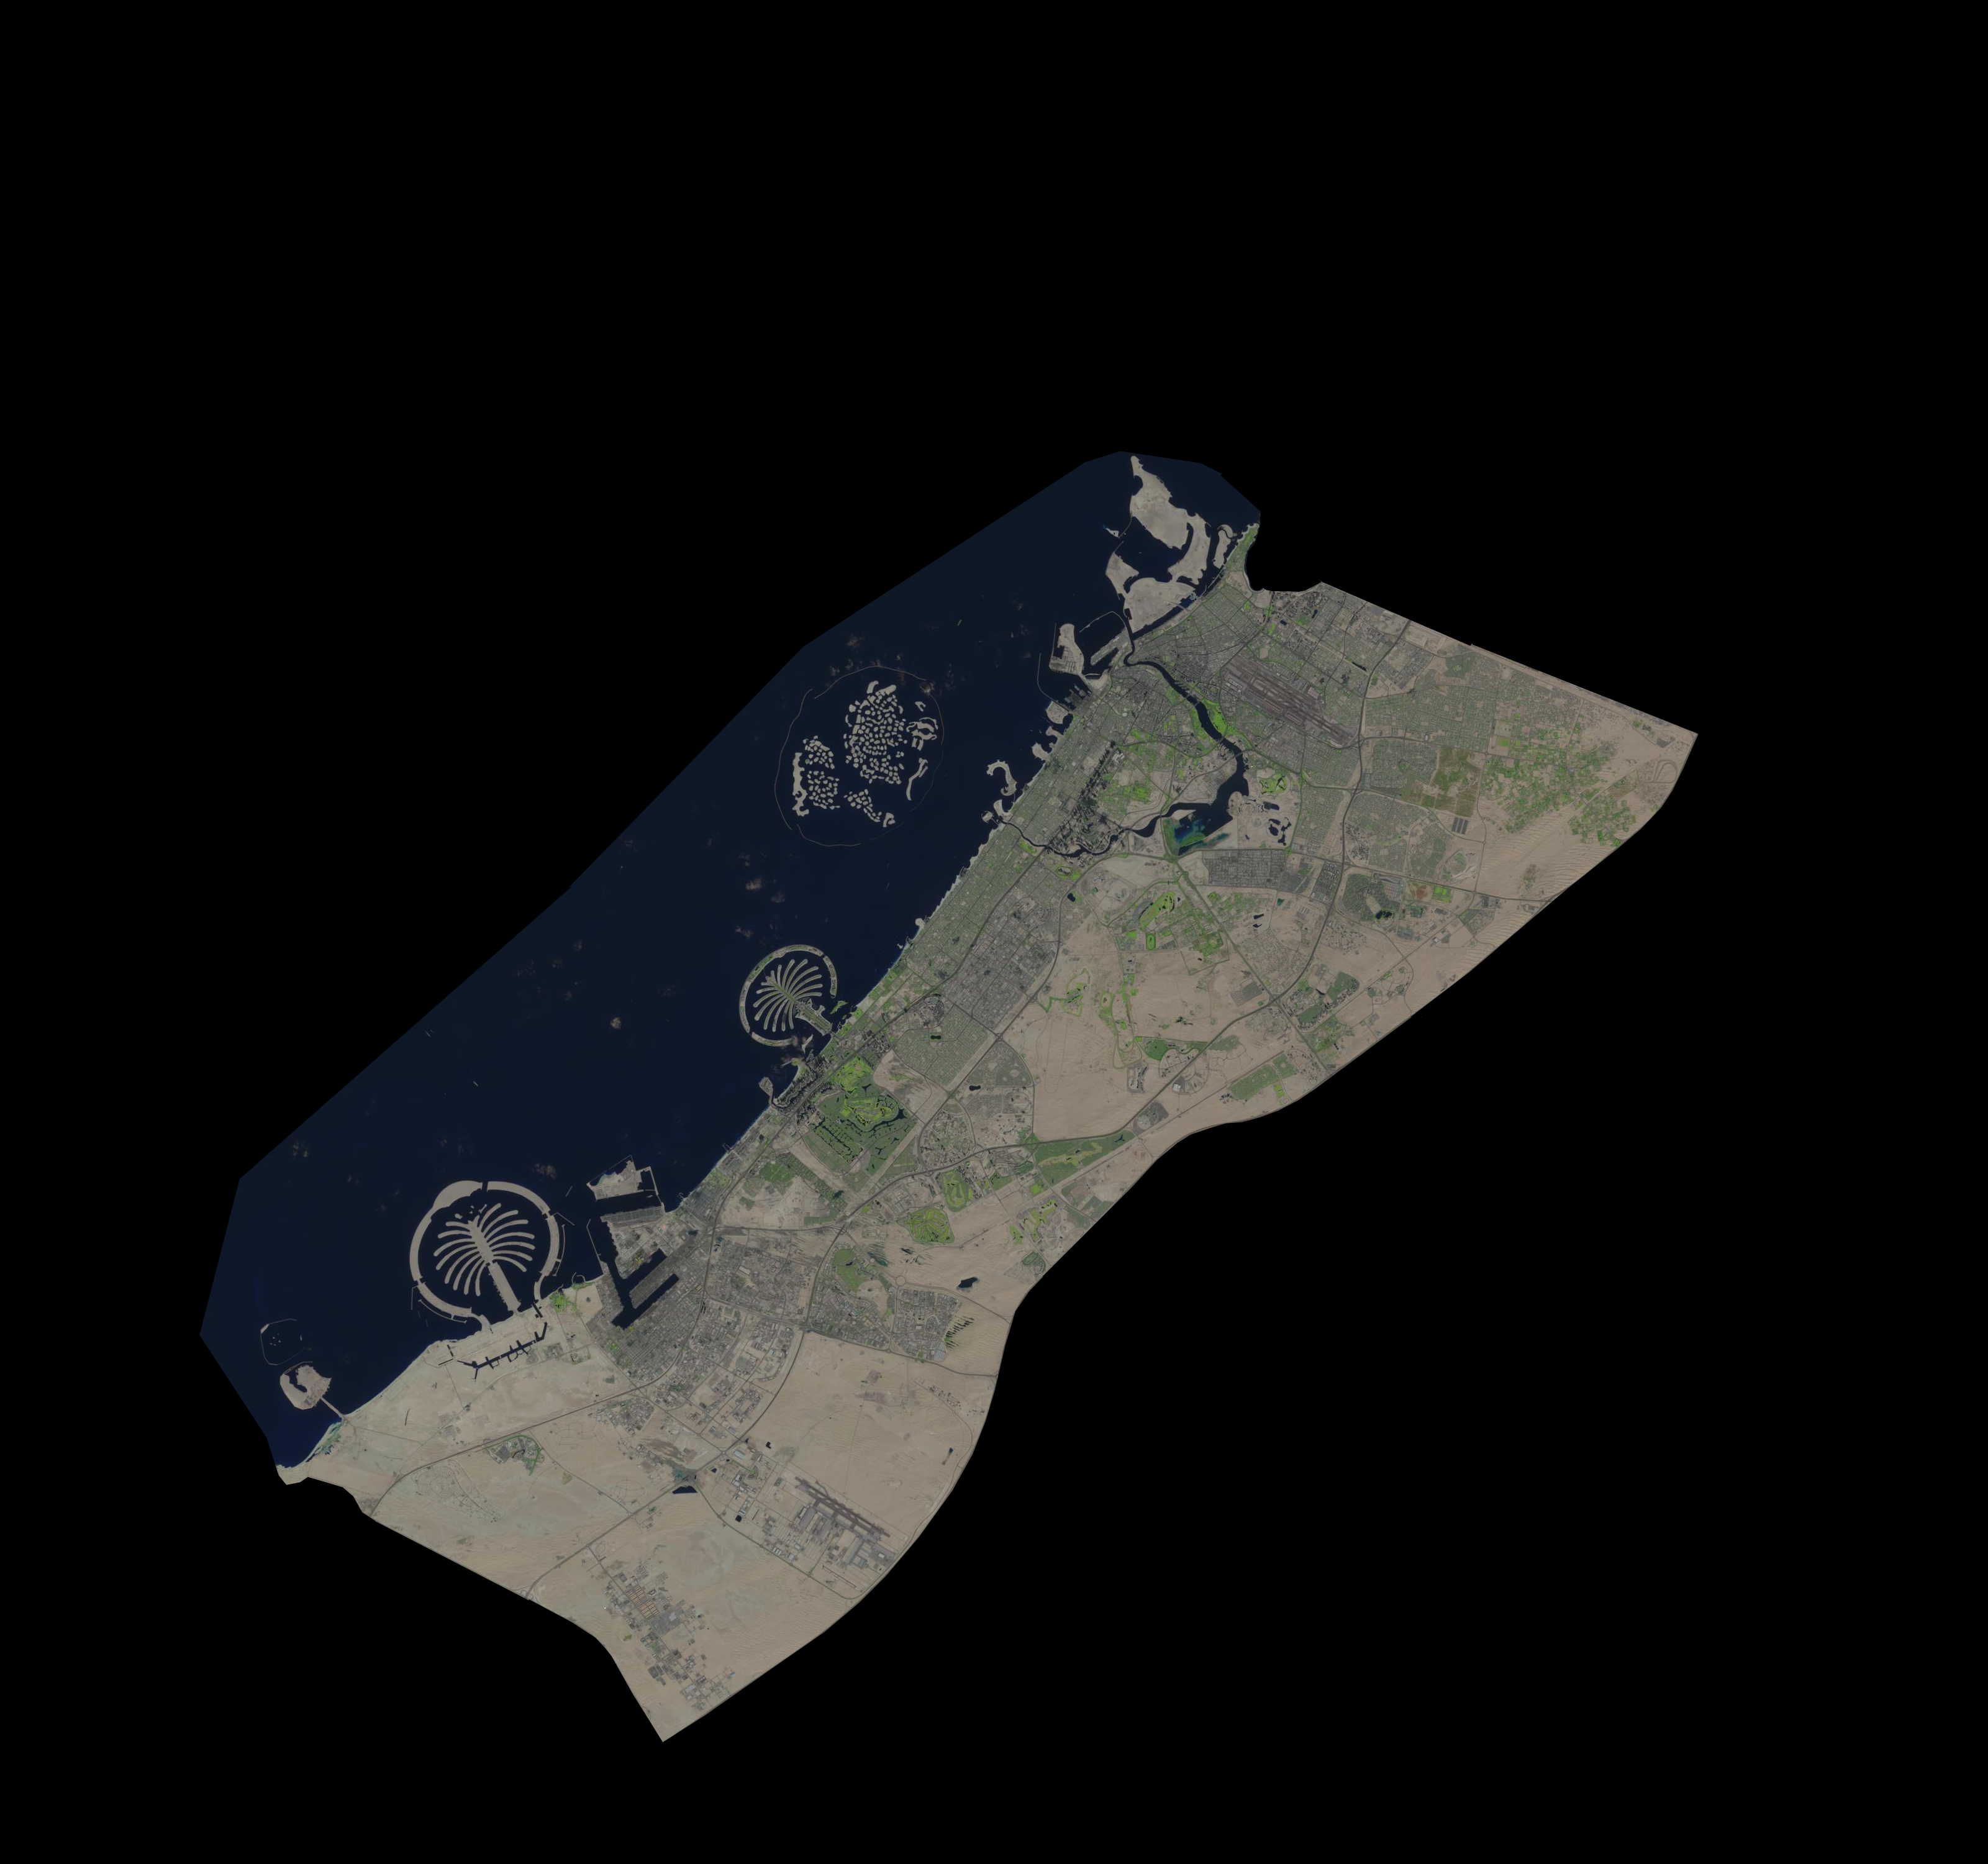
\includegraphics[width=\textwidth-3em]{code/imagedata/alldata/2016cropped}
	\caption{L-8 OLI Image (2016) cropped}
	\label{fig:L8OLI_16_cropped}
\end{minipage}%
\begin{minipage}{.5\textwidth}
	\centering
	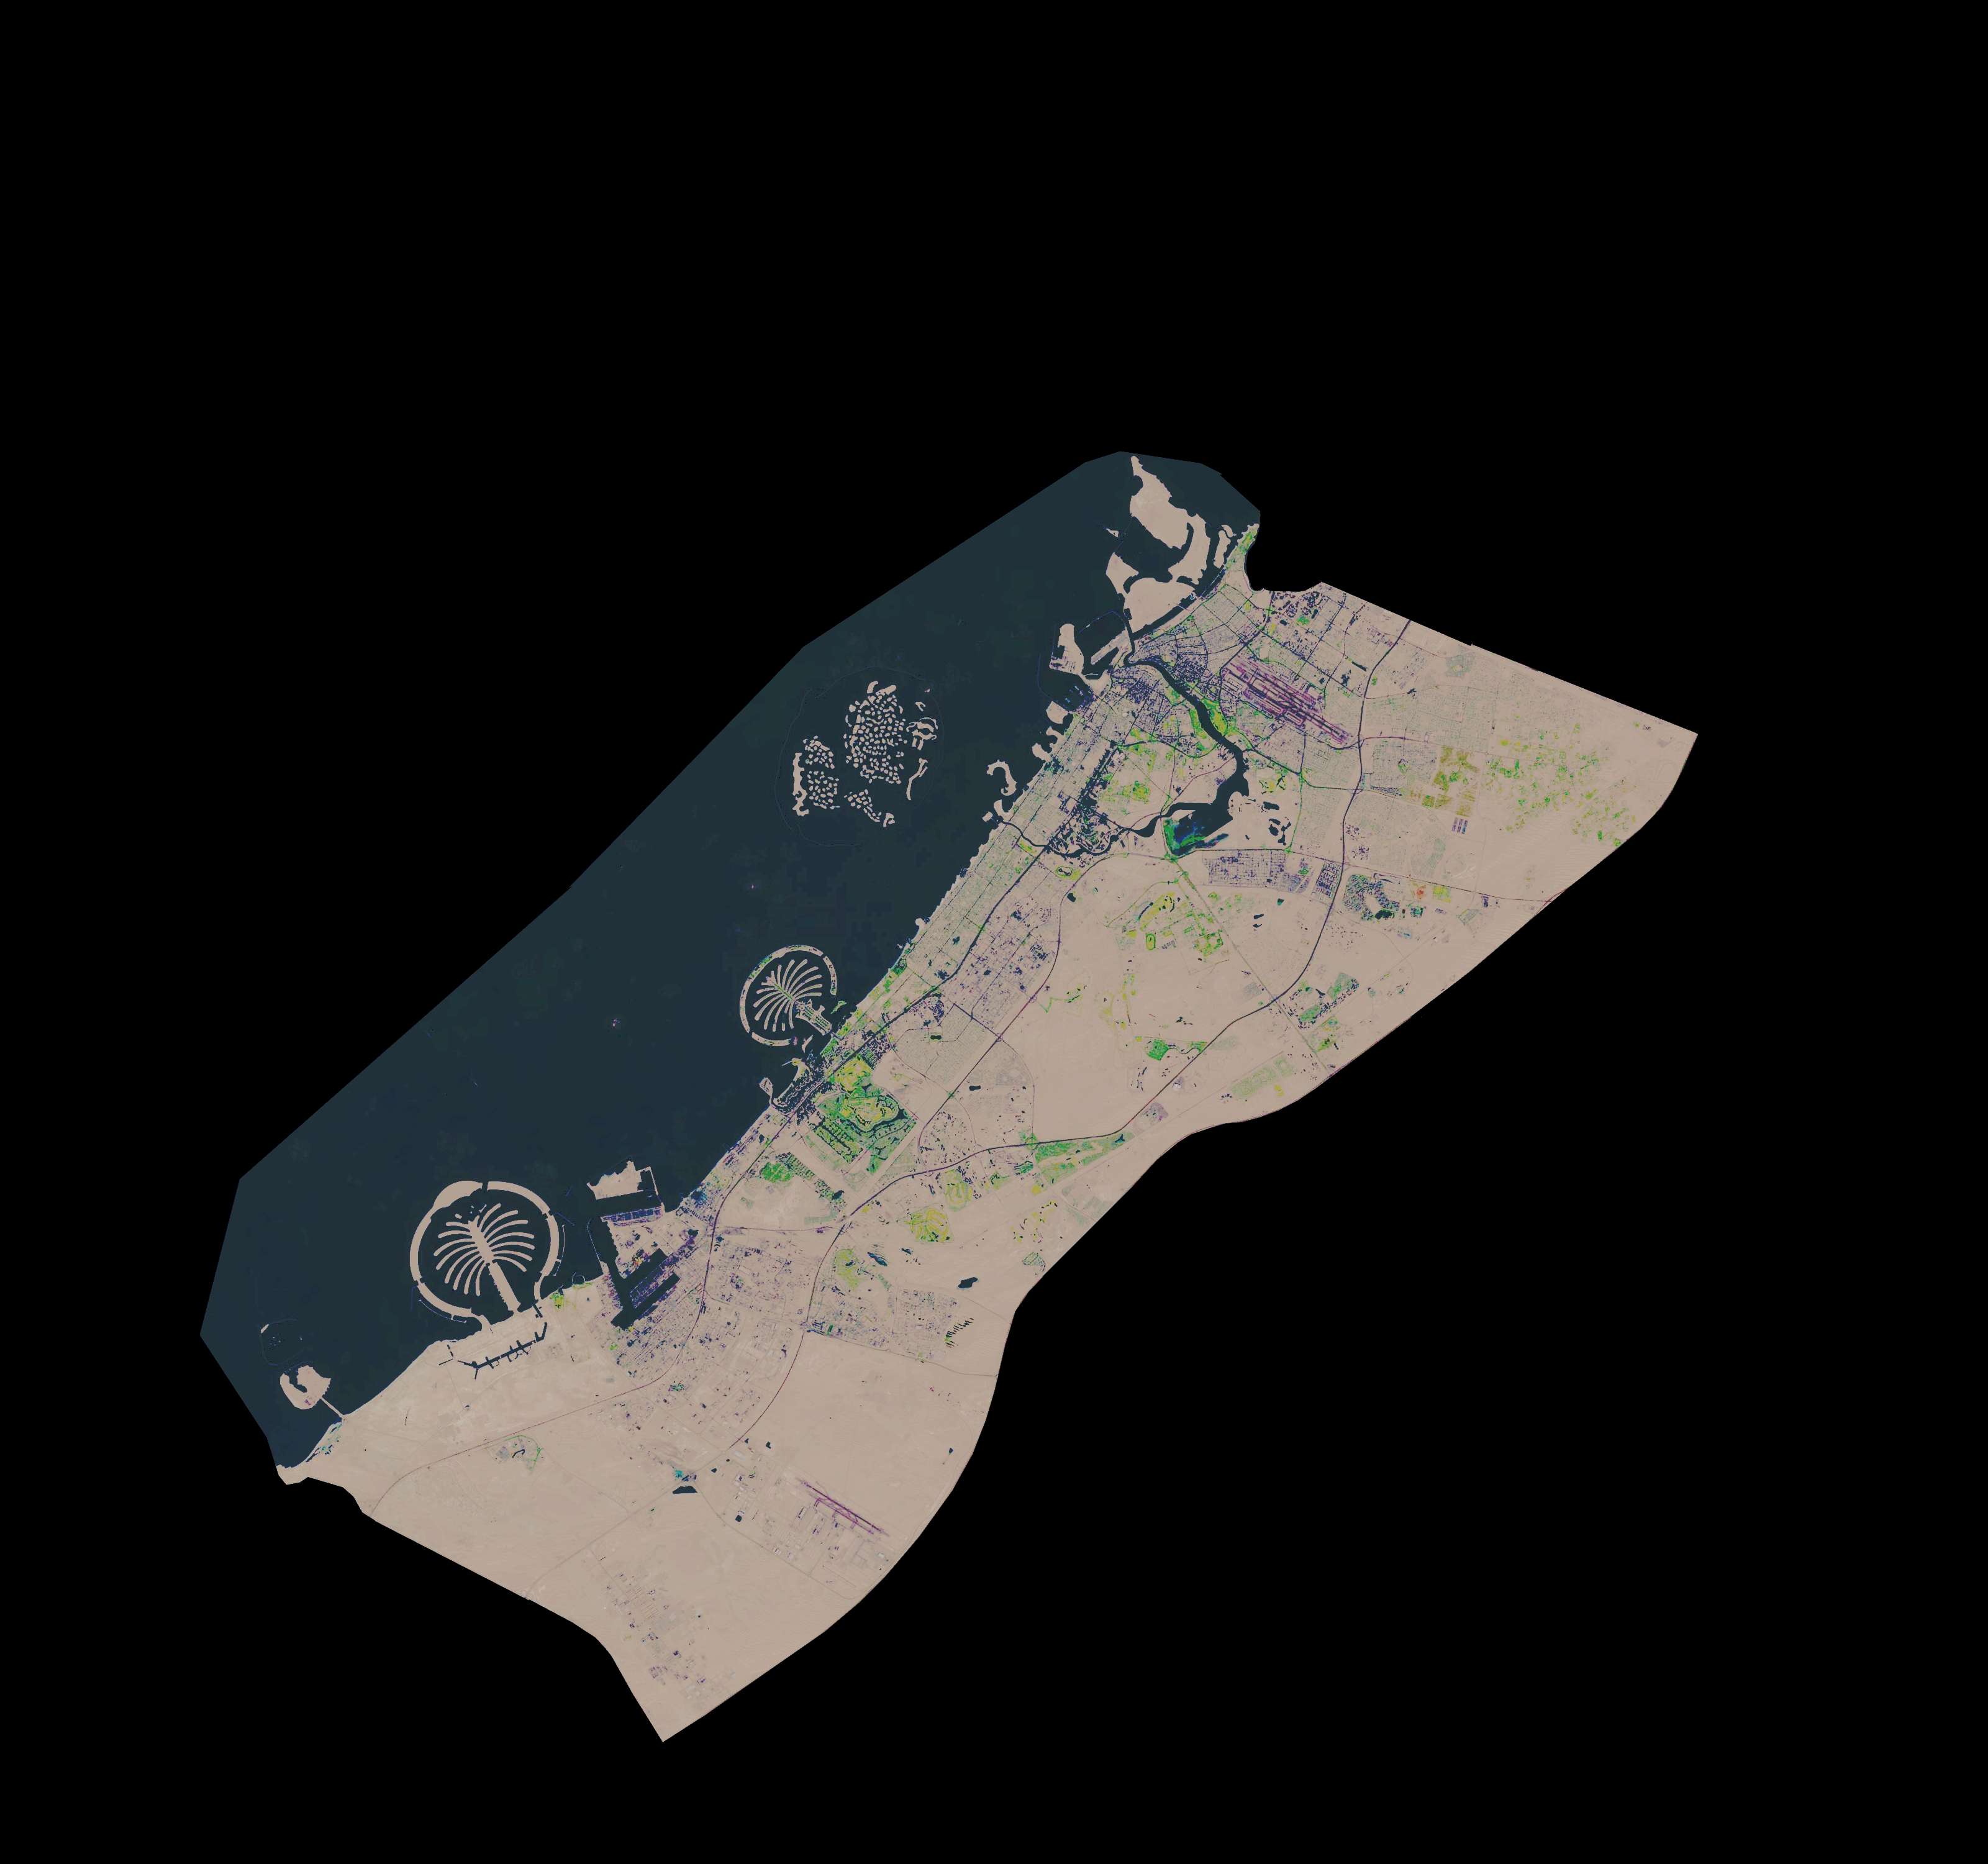
\includegraphics[width=\textwidth-3em]{code/imagedata/alldata/2016cropped_refd}
	\caption{L-8 OLI Image (2016) equalized}
	\label{fig:L8_OLI_16_equalised}
\end{minipage}
\end{figure}


\subsection{Structure Detection}
The now masked, cropped and equalised images could then be used for machine based processing. To prove or disprove the first hypotheses, the MATLAB built-in edge detection was used with some morphological filters. \\
First, the images are grayscaled with the MATLAB function \texttt{rgb2gray} (\cref{fig:greyscale}), then an edge-detection was performed with \texttt{edge} on the grayscaled image (\cref{fig:edge_detect}). Looking at the image resulting from this step, it can be seen that also the borders at the masked area are detected, which is not desired because we are not interested in the mask border. To remove the outer detected edges, a morphologic erosion is performed with the parameter of 1 pixel (meaning only 1 pixel will be eroded) (\cref{fig:morpherode}). \\
Since the edge detection only detected the edges, and not for example the inner part of a rectangle (assuming the rectangle being a house, or street), a morphological closing was performed to close those inner parts with a logical 1 (\cref{fig:morphclose}) (corresponding to the white colour in the binary images). Different edge detection algorithms were tested, e.g. Canny, but the build-in edge function provided the best results in terms of detecting the desired features (mostly streets/houses etc.). Also, the parameters for the morphological closing were chosen as \textit{Infinite}, since a complete closure of the \todo{eingeschlossenen} areas was desired.\\
After having obtained the masked area corresponding to streets, houses and other structured elements, the area could be calculated by simply summing the binary image.


\begin{figure}[h!]
\centering
\begin{minipage}{.5\textwidth}
	\centering
	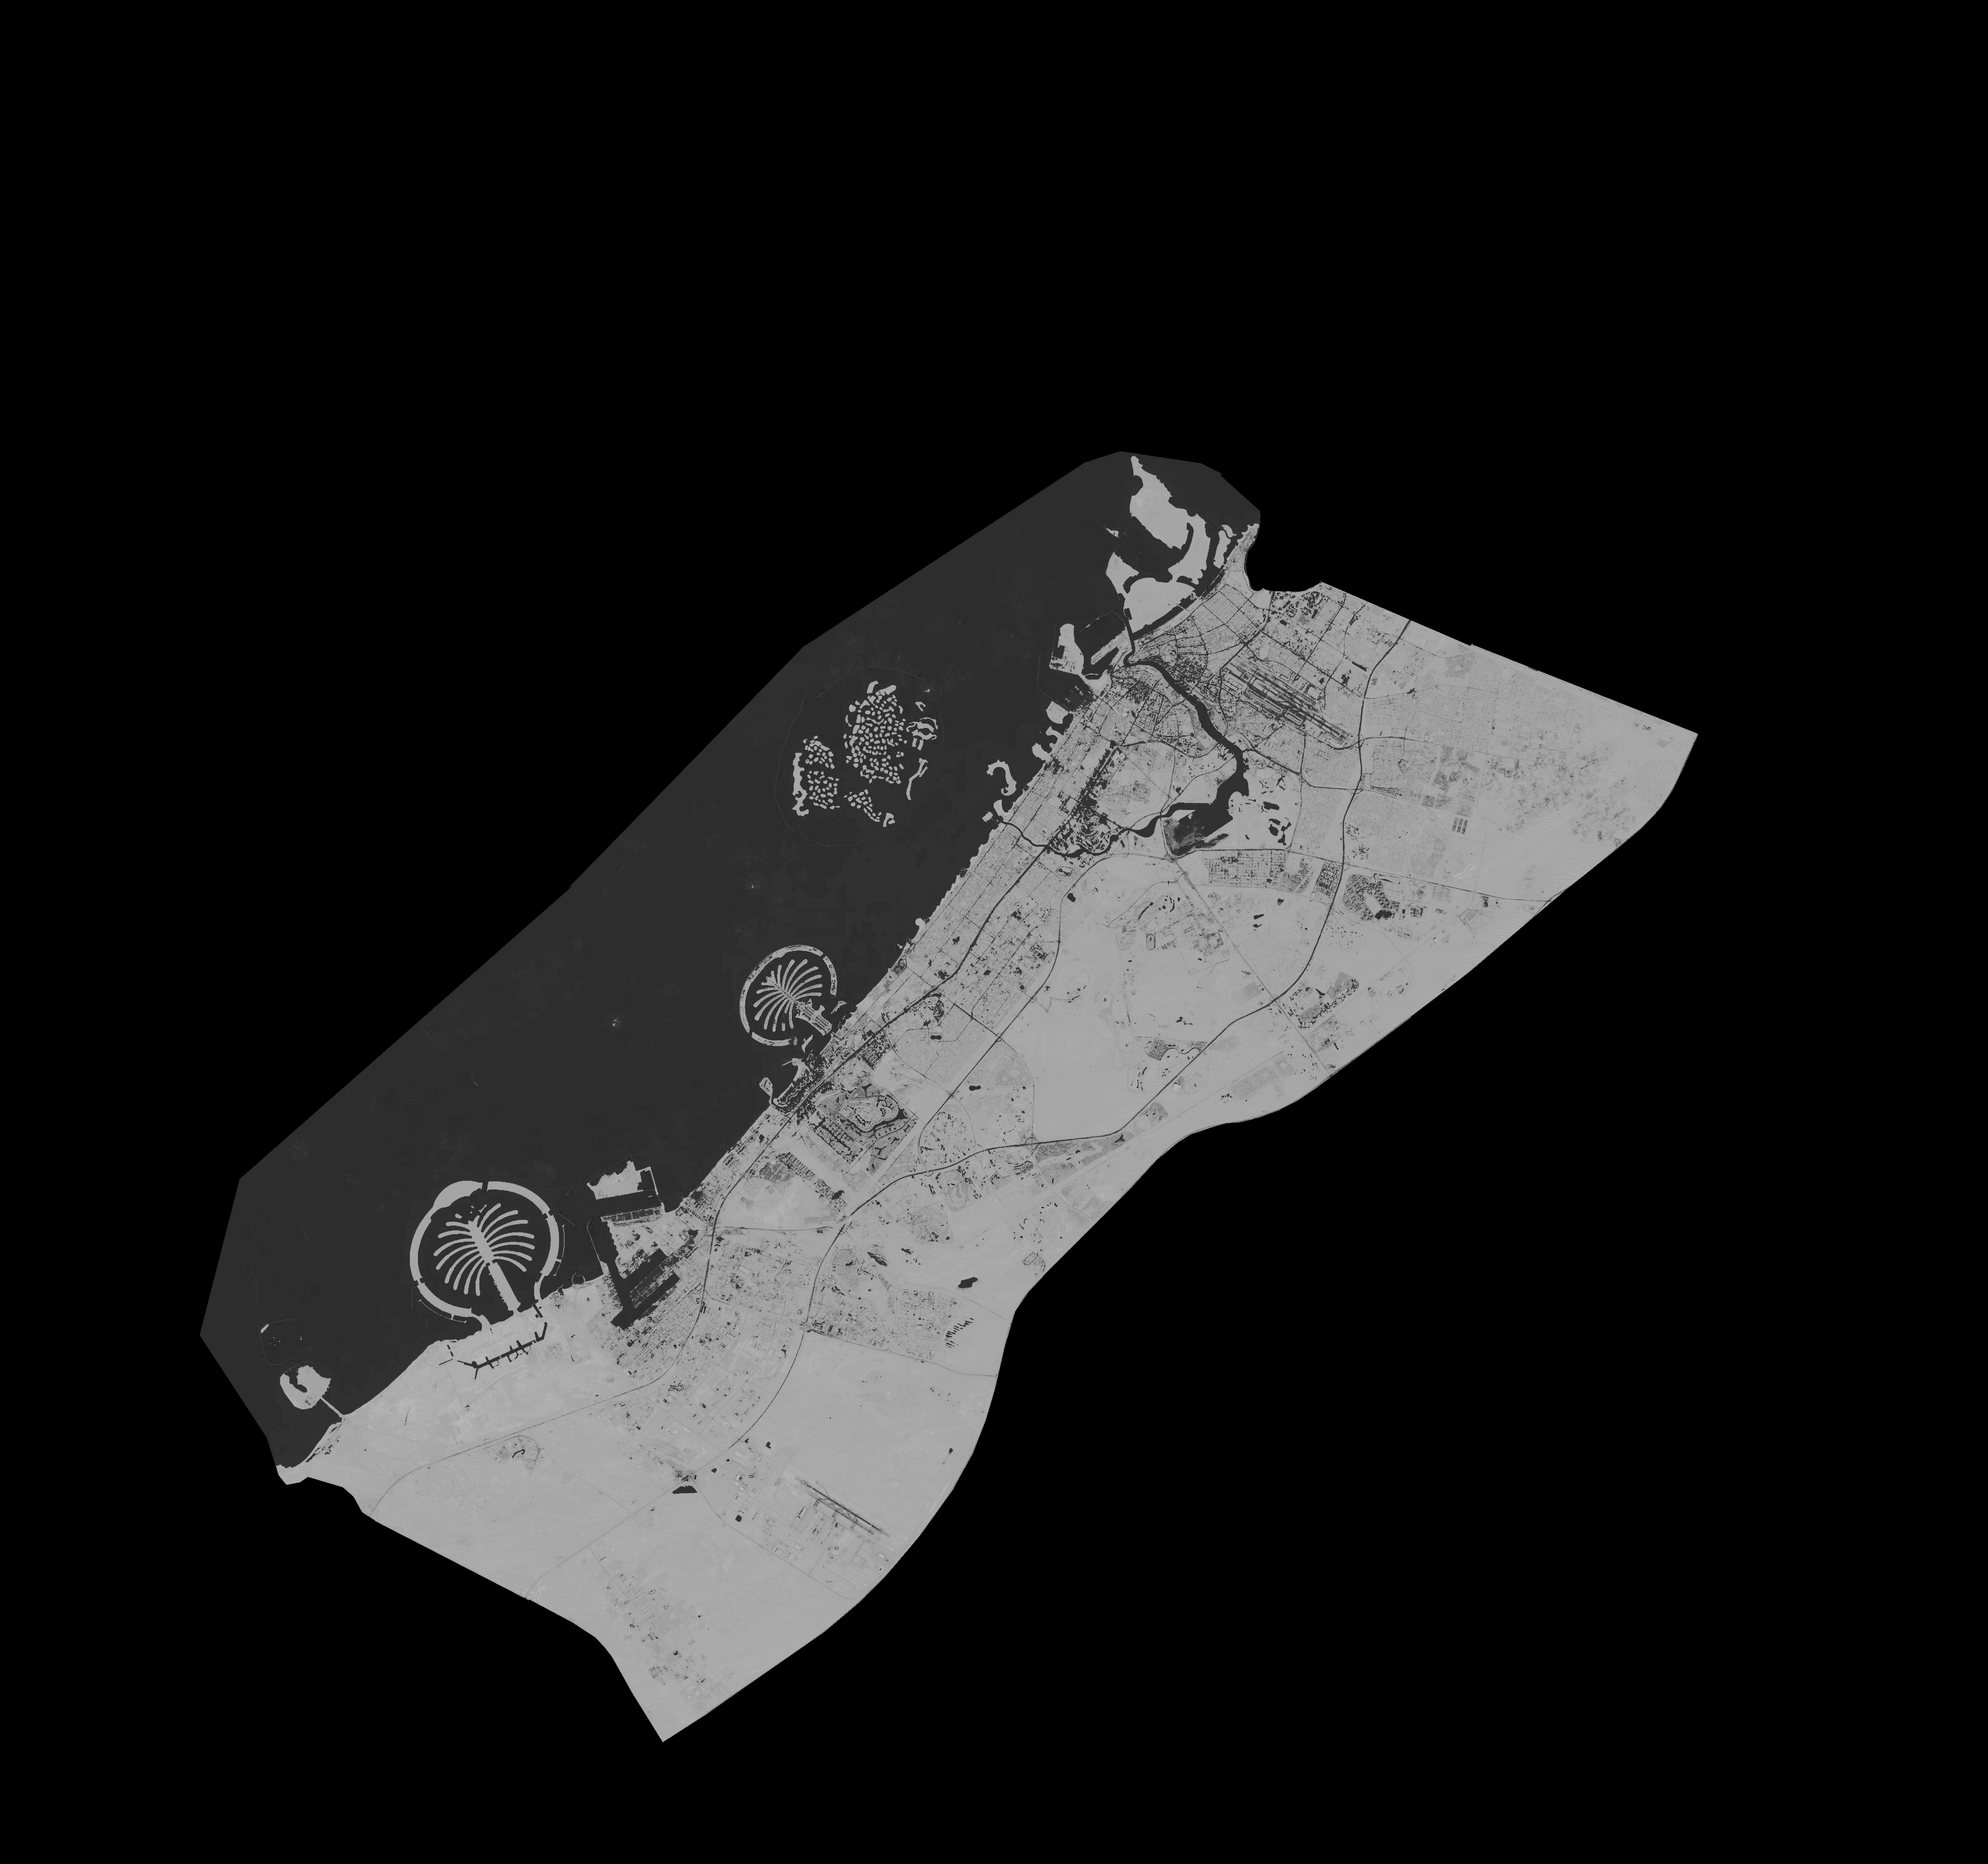
\includegraphics[width=\textwidth-3em]{code/imagedata/analysis/street2016cropped_refd_grayscale}
	\caption{L-8 OLI Image (2016) grayscaled}
	\label{fig:greyscale}
\end{minipage}%
\begin{minipage}{.5\textwidth}
	\centering
	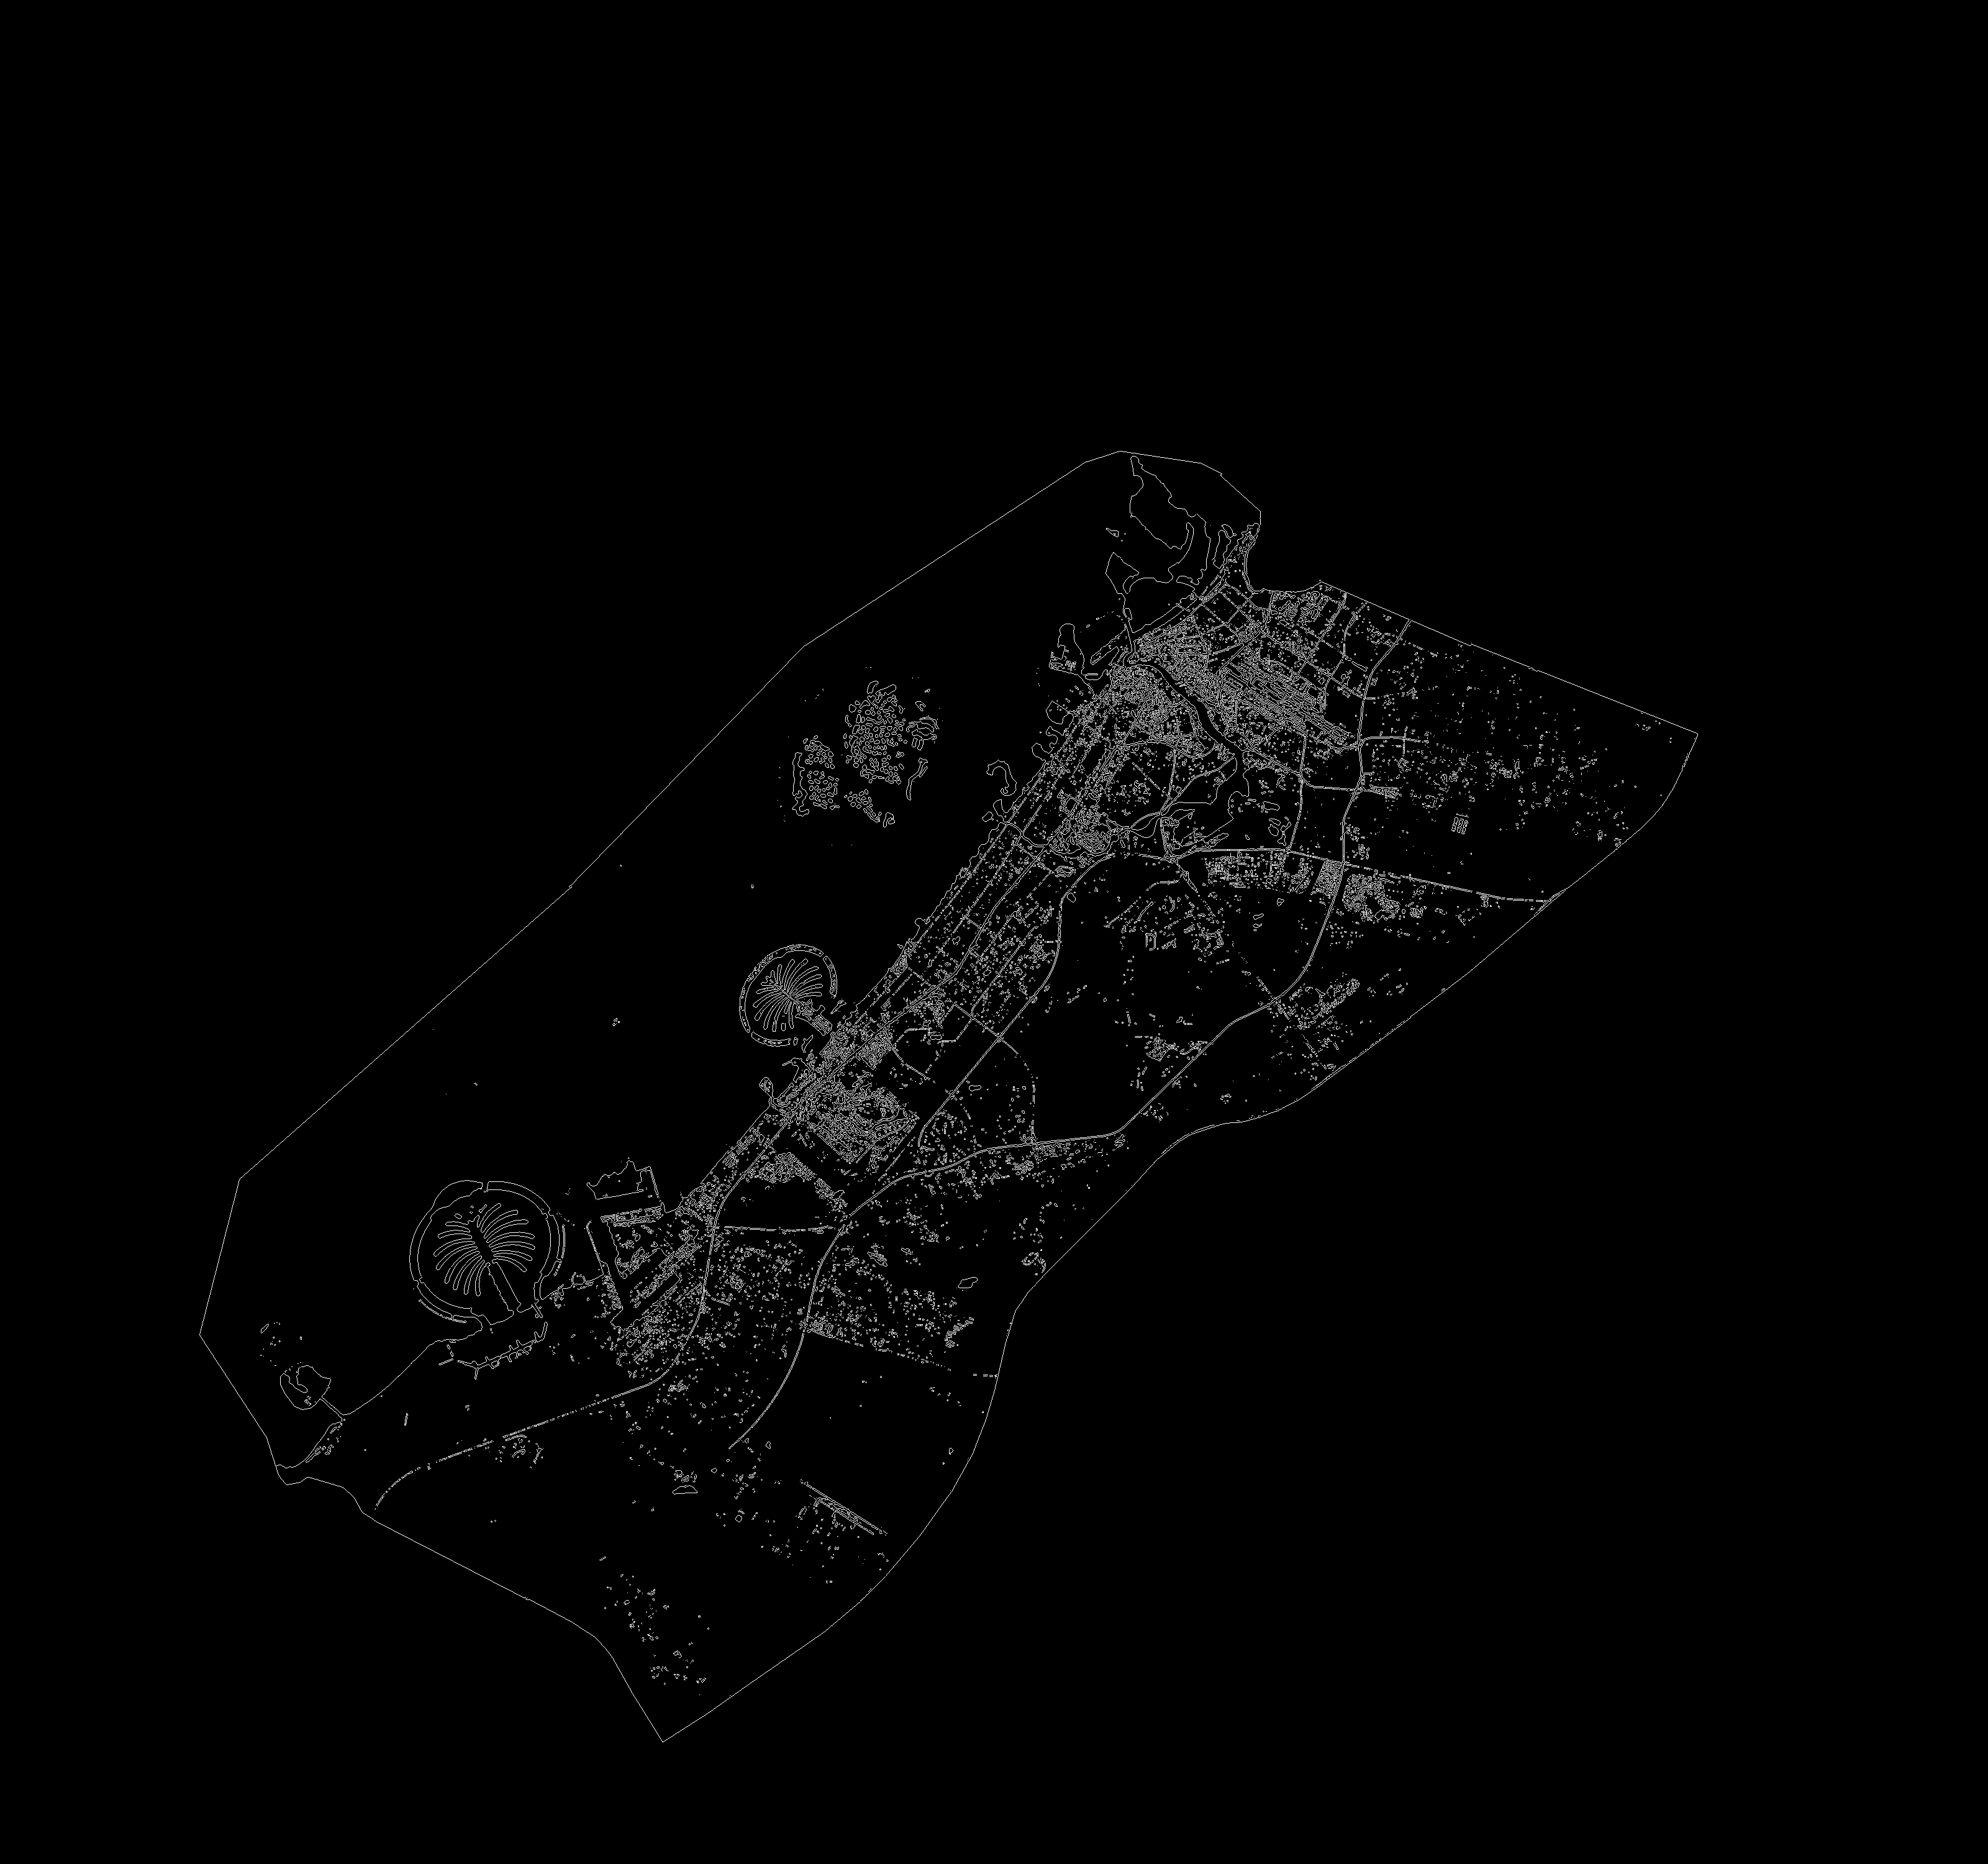
\includegraphics[width=\textwidth-3em]{code/imagedata/analysis/street2016cropped_refd_edge}
	\caption{L-8 OLI Image (2016) edge detection}
	\label{fig:edge_detect}
\end{minipage}
\end{figure}

\begin{figure}[h!]
\centering
\begin{minipage}{.5\textwidth}
	\centering
	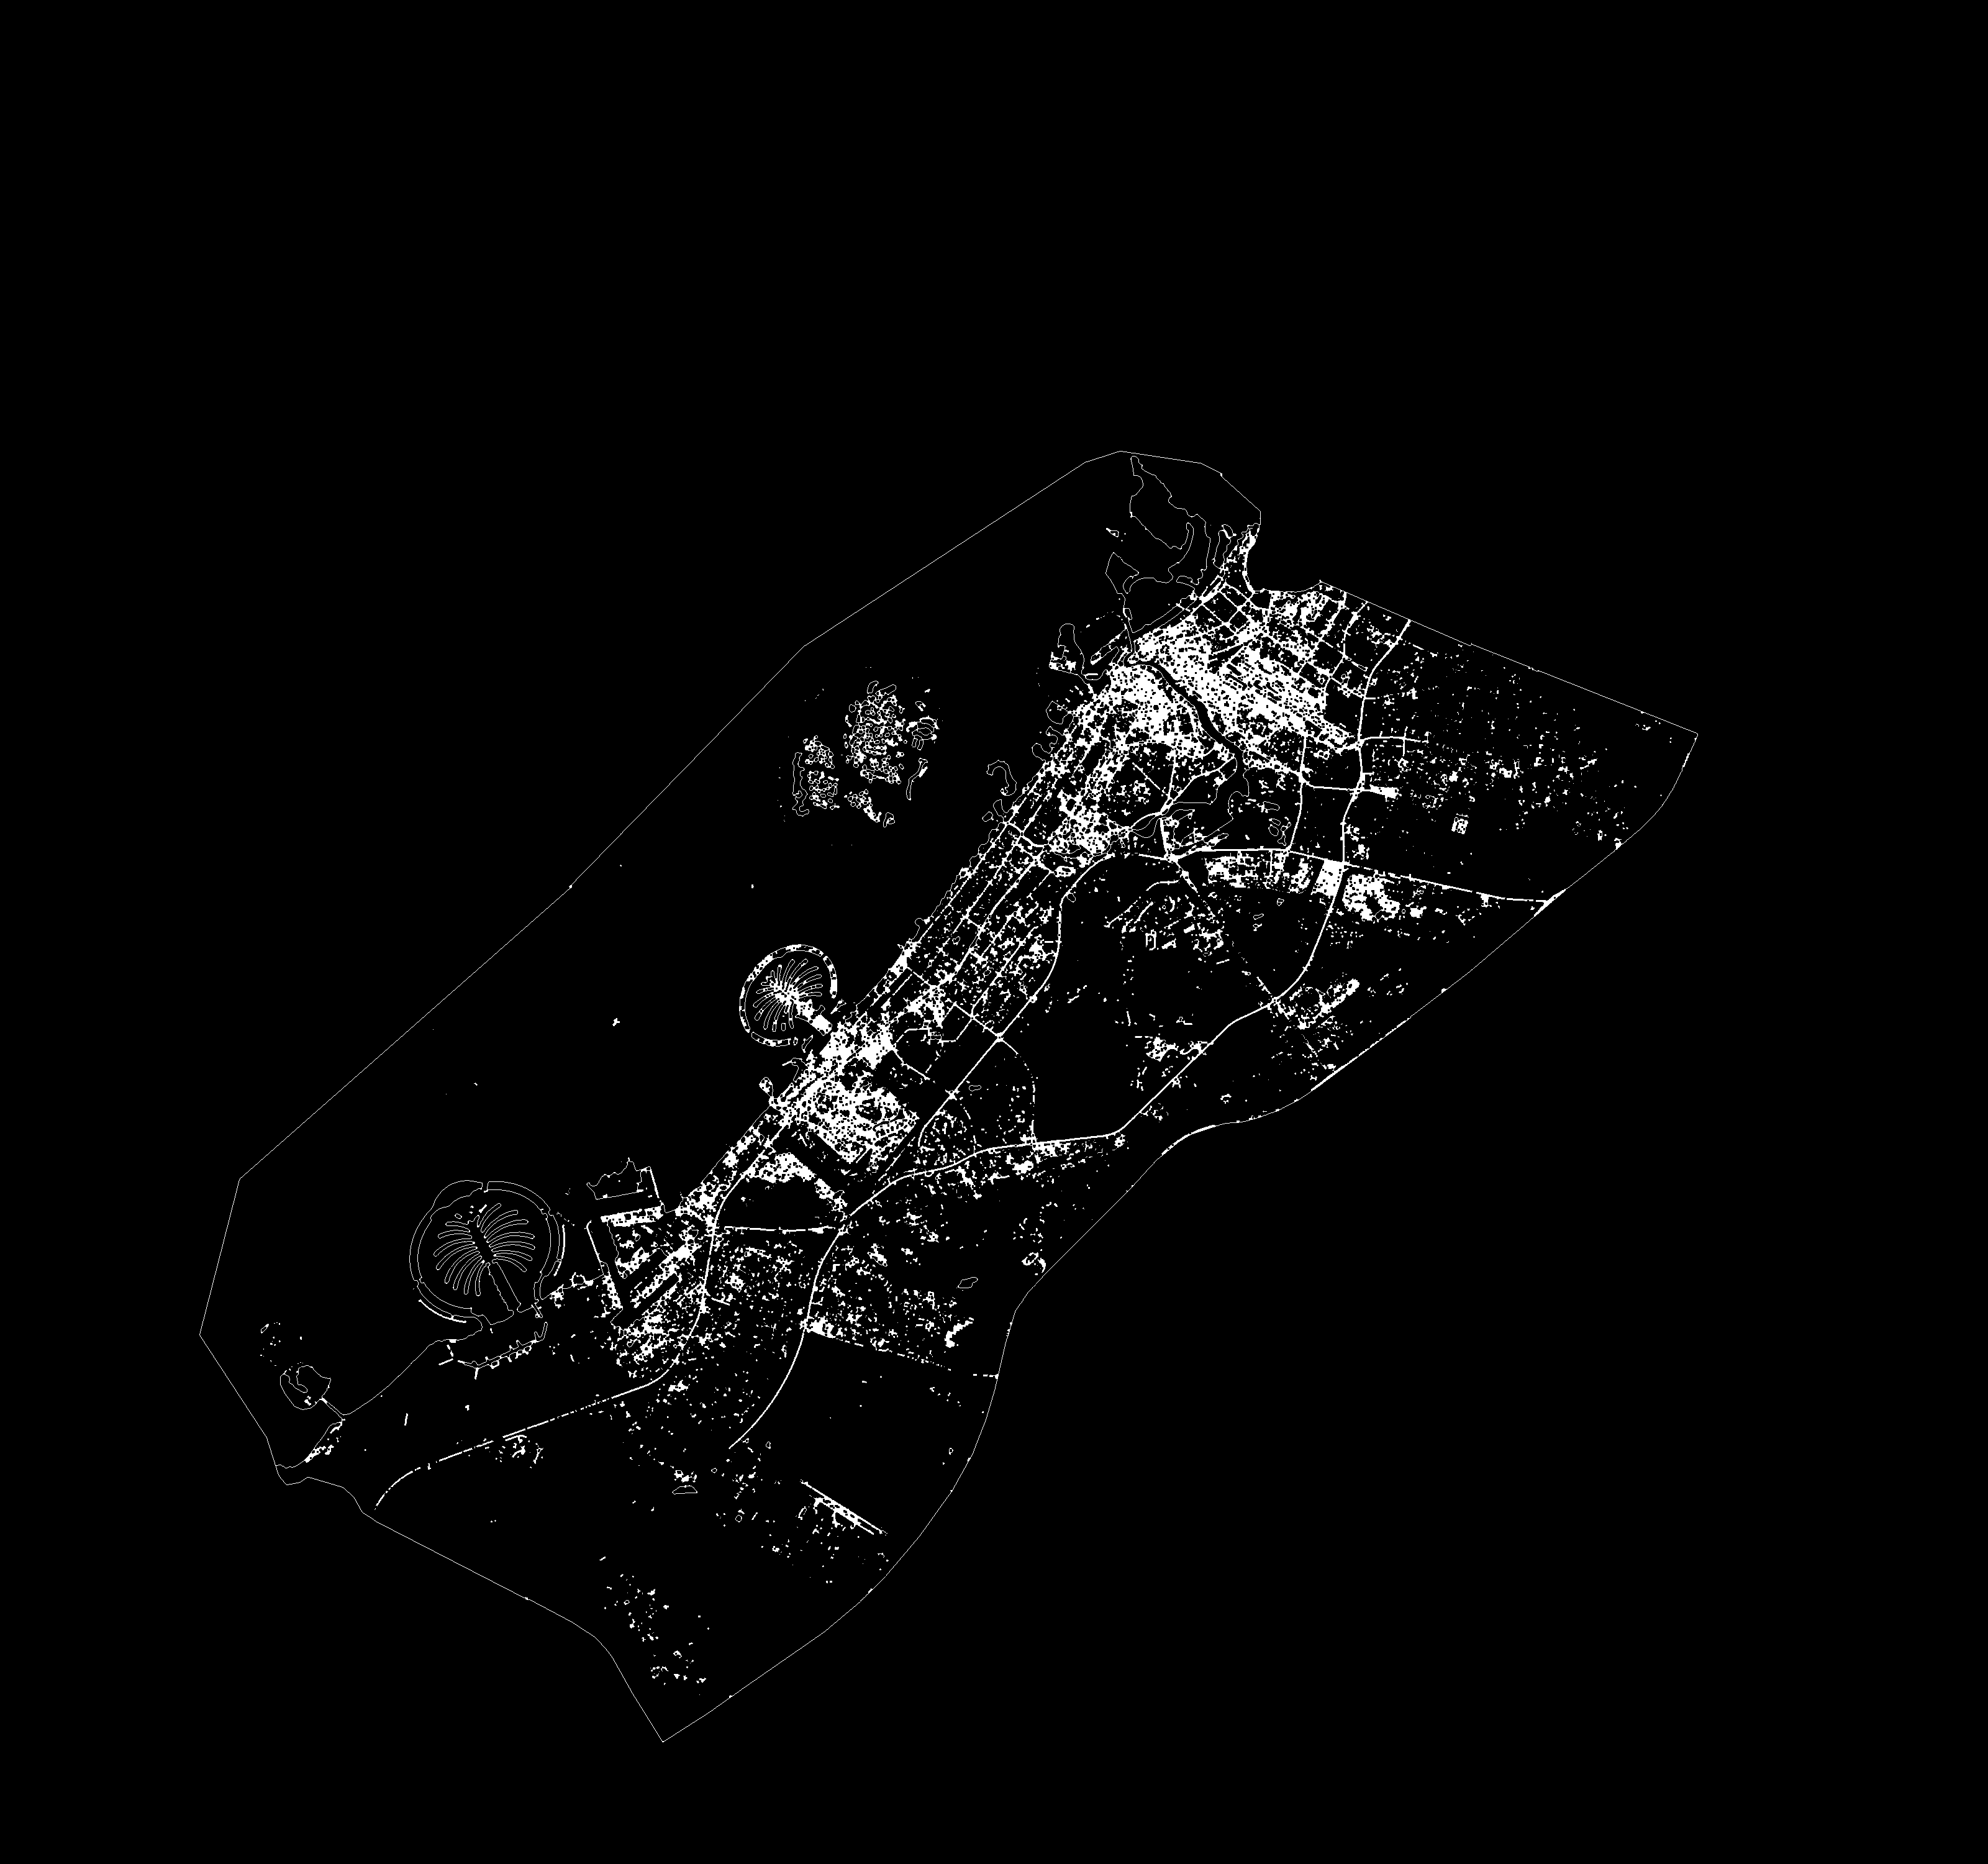
\includegraphics[width=\textwidth-3em]{code/imagedata/analysis/street2016cropped_refd_close}
	\caption{L-8 OLI Image (2016) morph. closing}
	\label{fig:morphclose}
\end{minipage}%
\begin{minipage}{.5\textwidth}
	\centering
	
\includegraphics[width=\textwidth-3em]{code/imagedata/analysis/street2016cropped_refd_erode}
	\caption{L-8 OLI Image (2016) eroded}
	\label{fig:morpherode}
\end{minipage}
\end{figure}

\subsection{Colour Analysis}
To obtain images that support or do not support the second hypothesis, a colour analysis of the image was necessary. As explained in \cref{subsec:pre}, the histograms of each distinct image were equalised to have comparable images.\\
The different image segments (e.g. vegetation, water, land) were then classified using supervised classification and the kNN-algorithm. For this, reference RGB values had to taken of the different desired classes to build a database for reference classes. This was done manually and the database then embedded in the MATLAB Code for the classification. For the purpose of this report only the results of the \textit{water}-class are used.
The algorithm was then run on the masked, cropped and equalised images (\cref{fig:L8_OLI_16_equalised}). Two example results can be seen in \cref{fig:water_2016,fig:water_1984}.

\begin{figure}[h!]
\centering
\begin{minipage}{.5\textwidth}
	\centering
	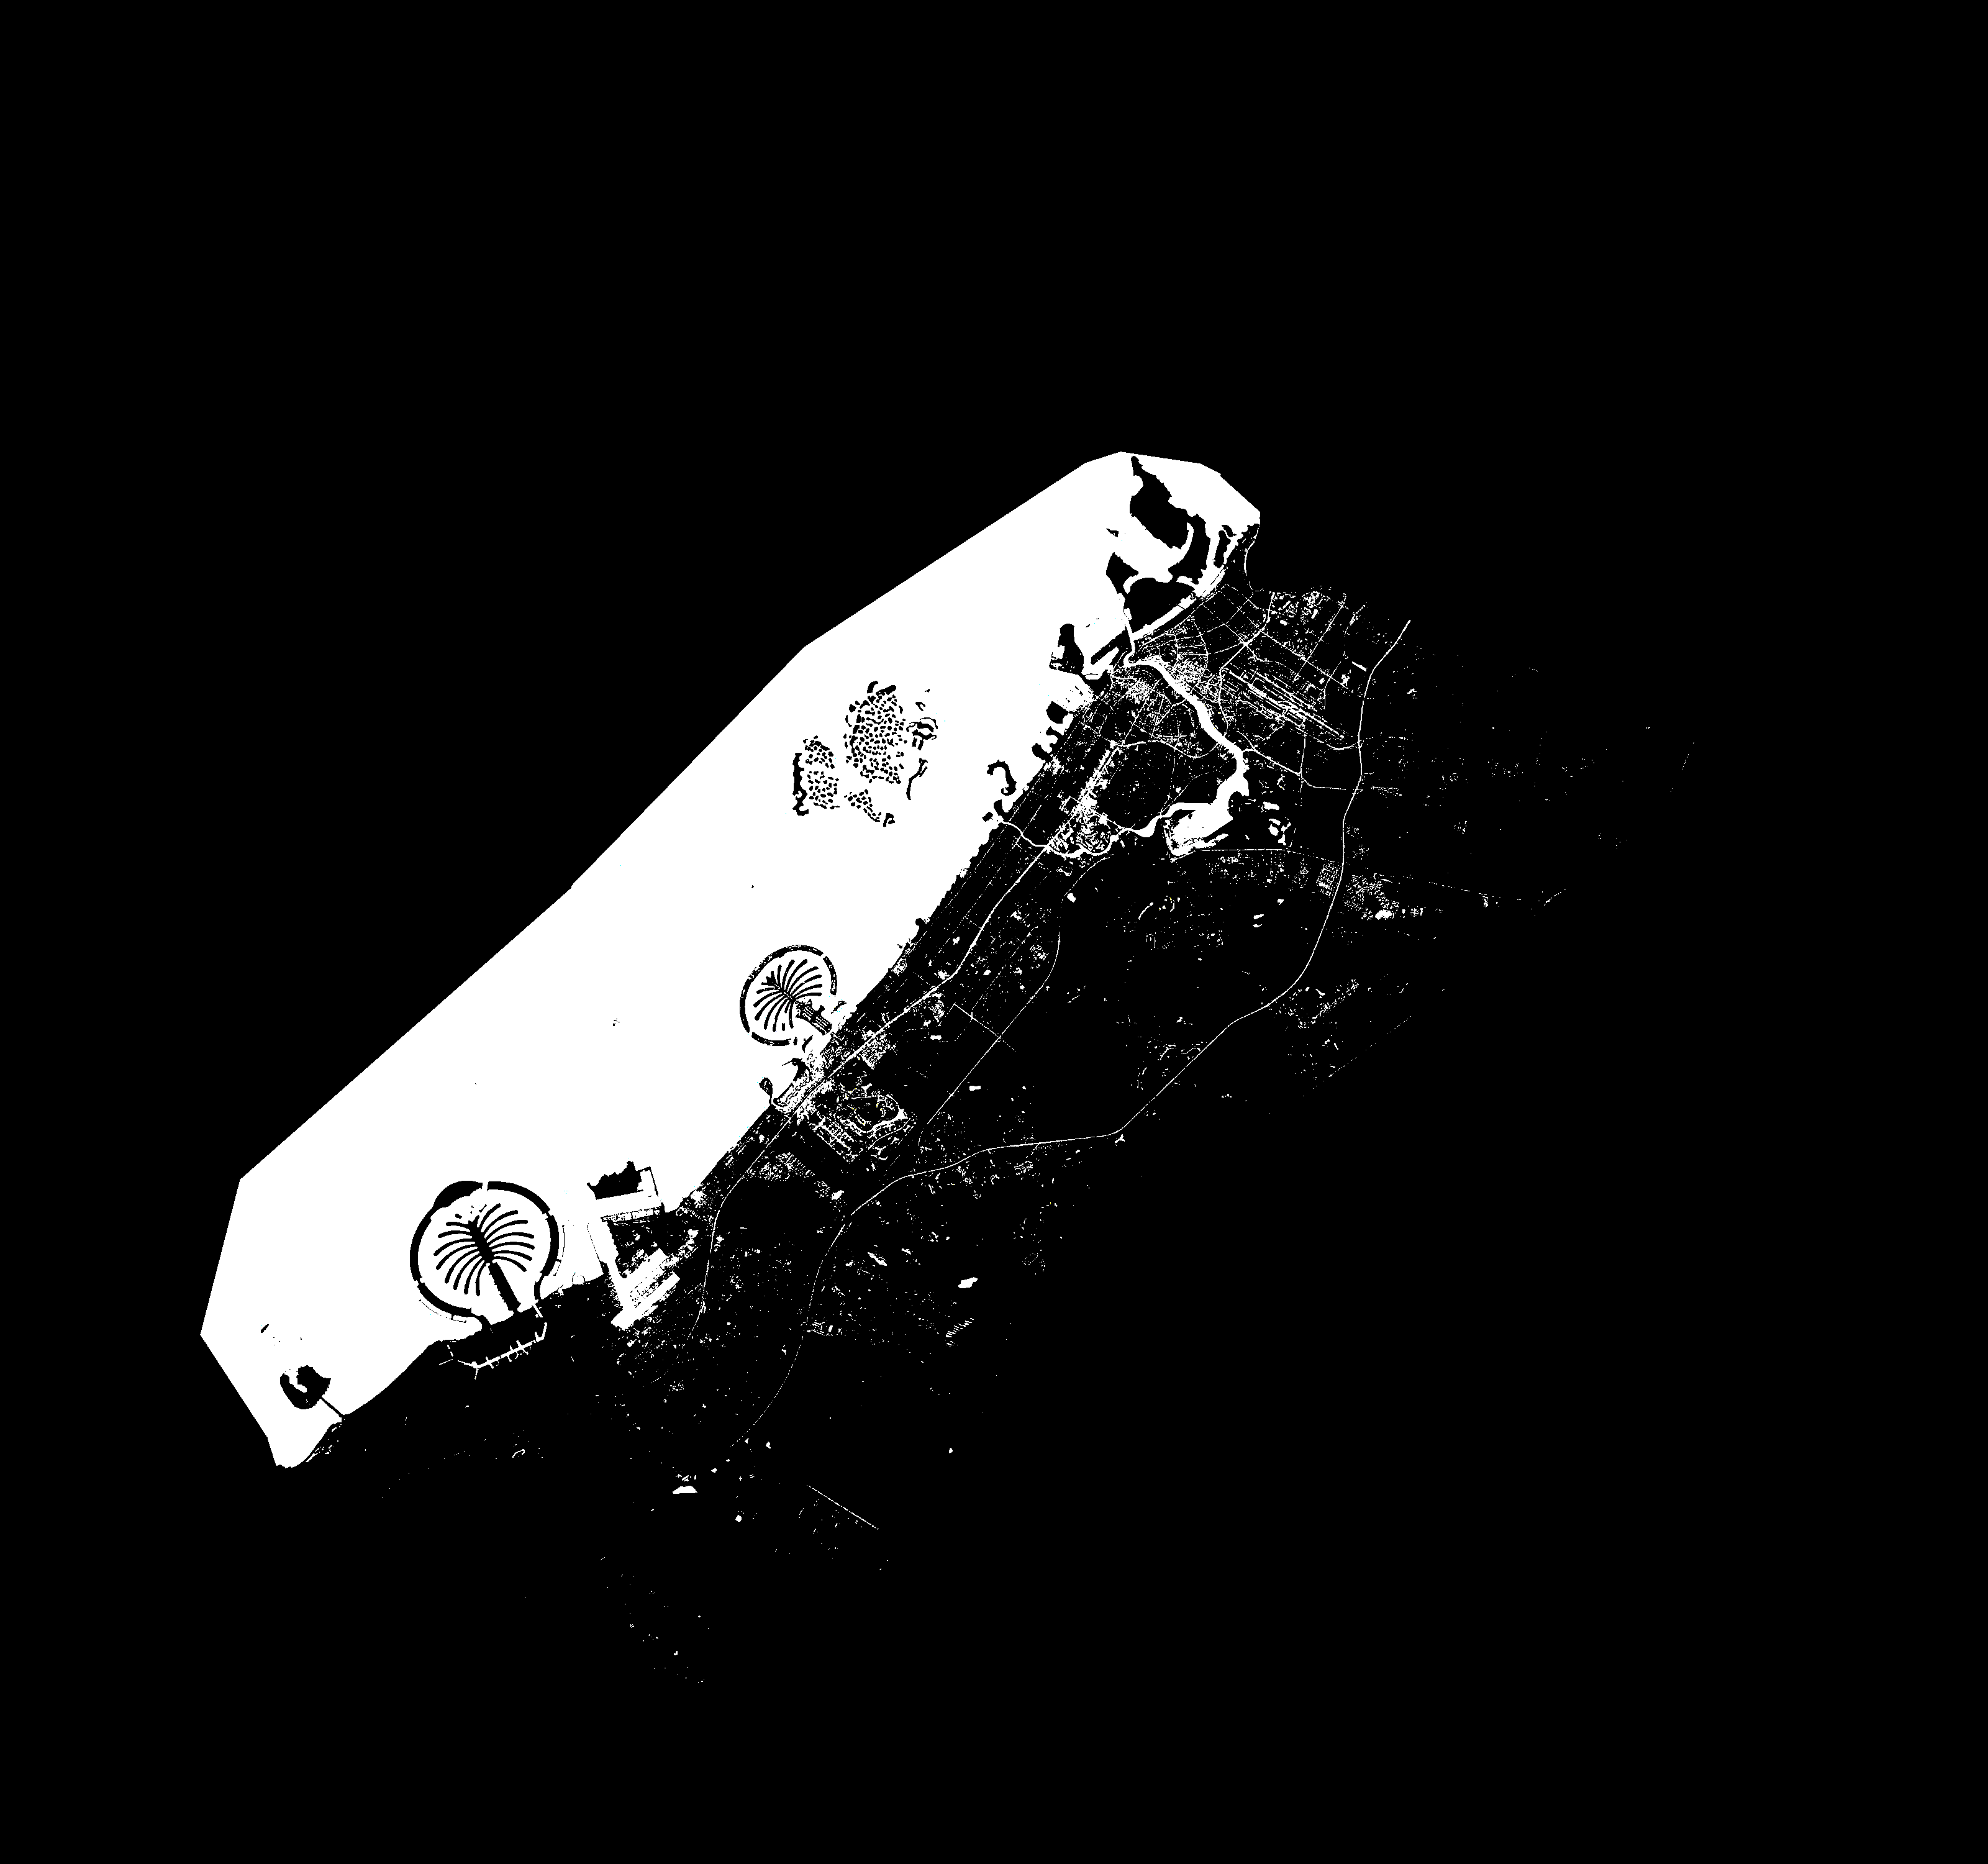
\includegraphics[width=\textwidth-3em]{code/imagedata/analysis/water2016cropped_refd_w}
	\caption{L-8 OLI Image (2016) water class}
	\label{fig:water_2016}
\end{minipage}%
\begin{minipage}{.5\textwidth}
	\centering
	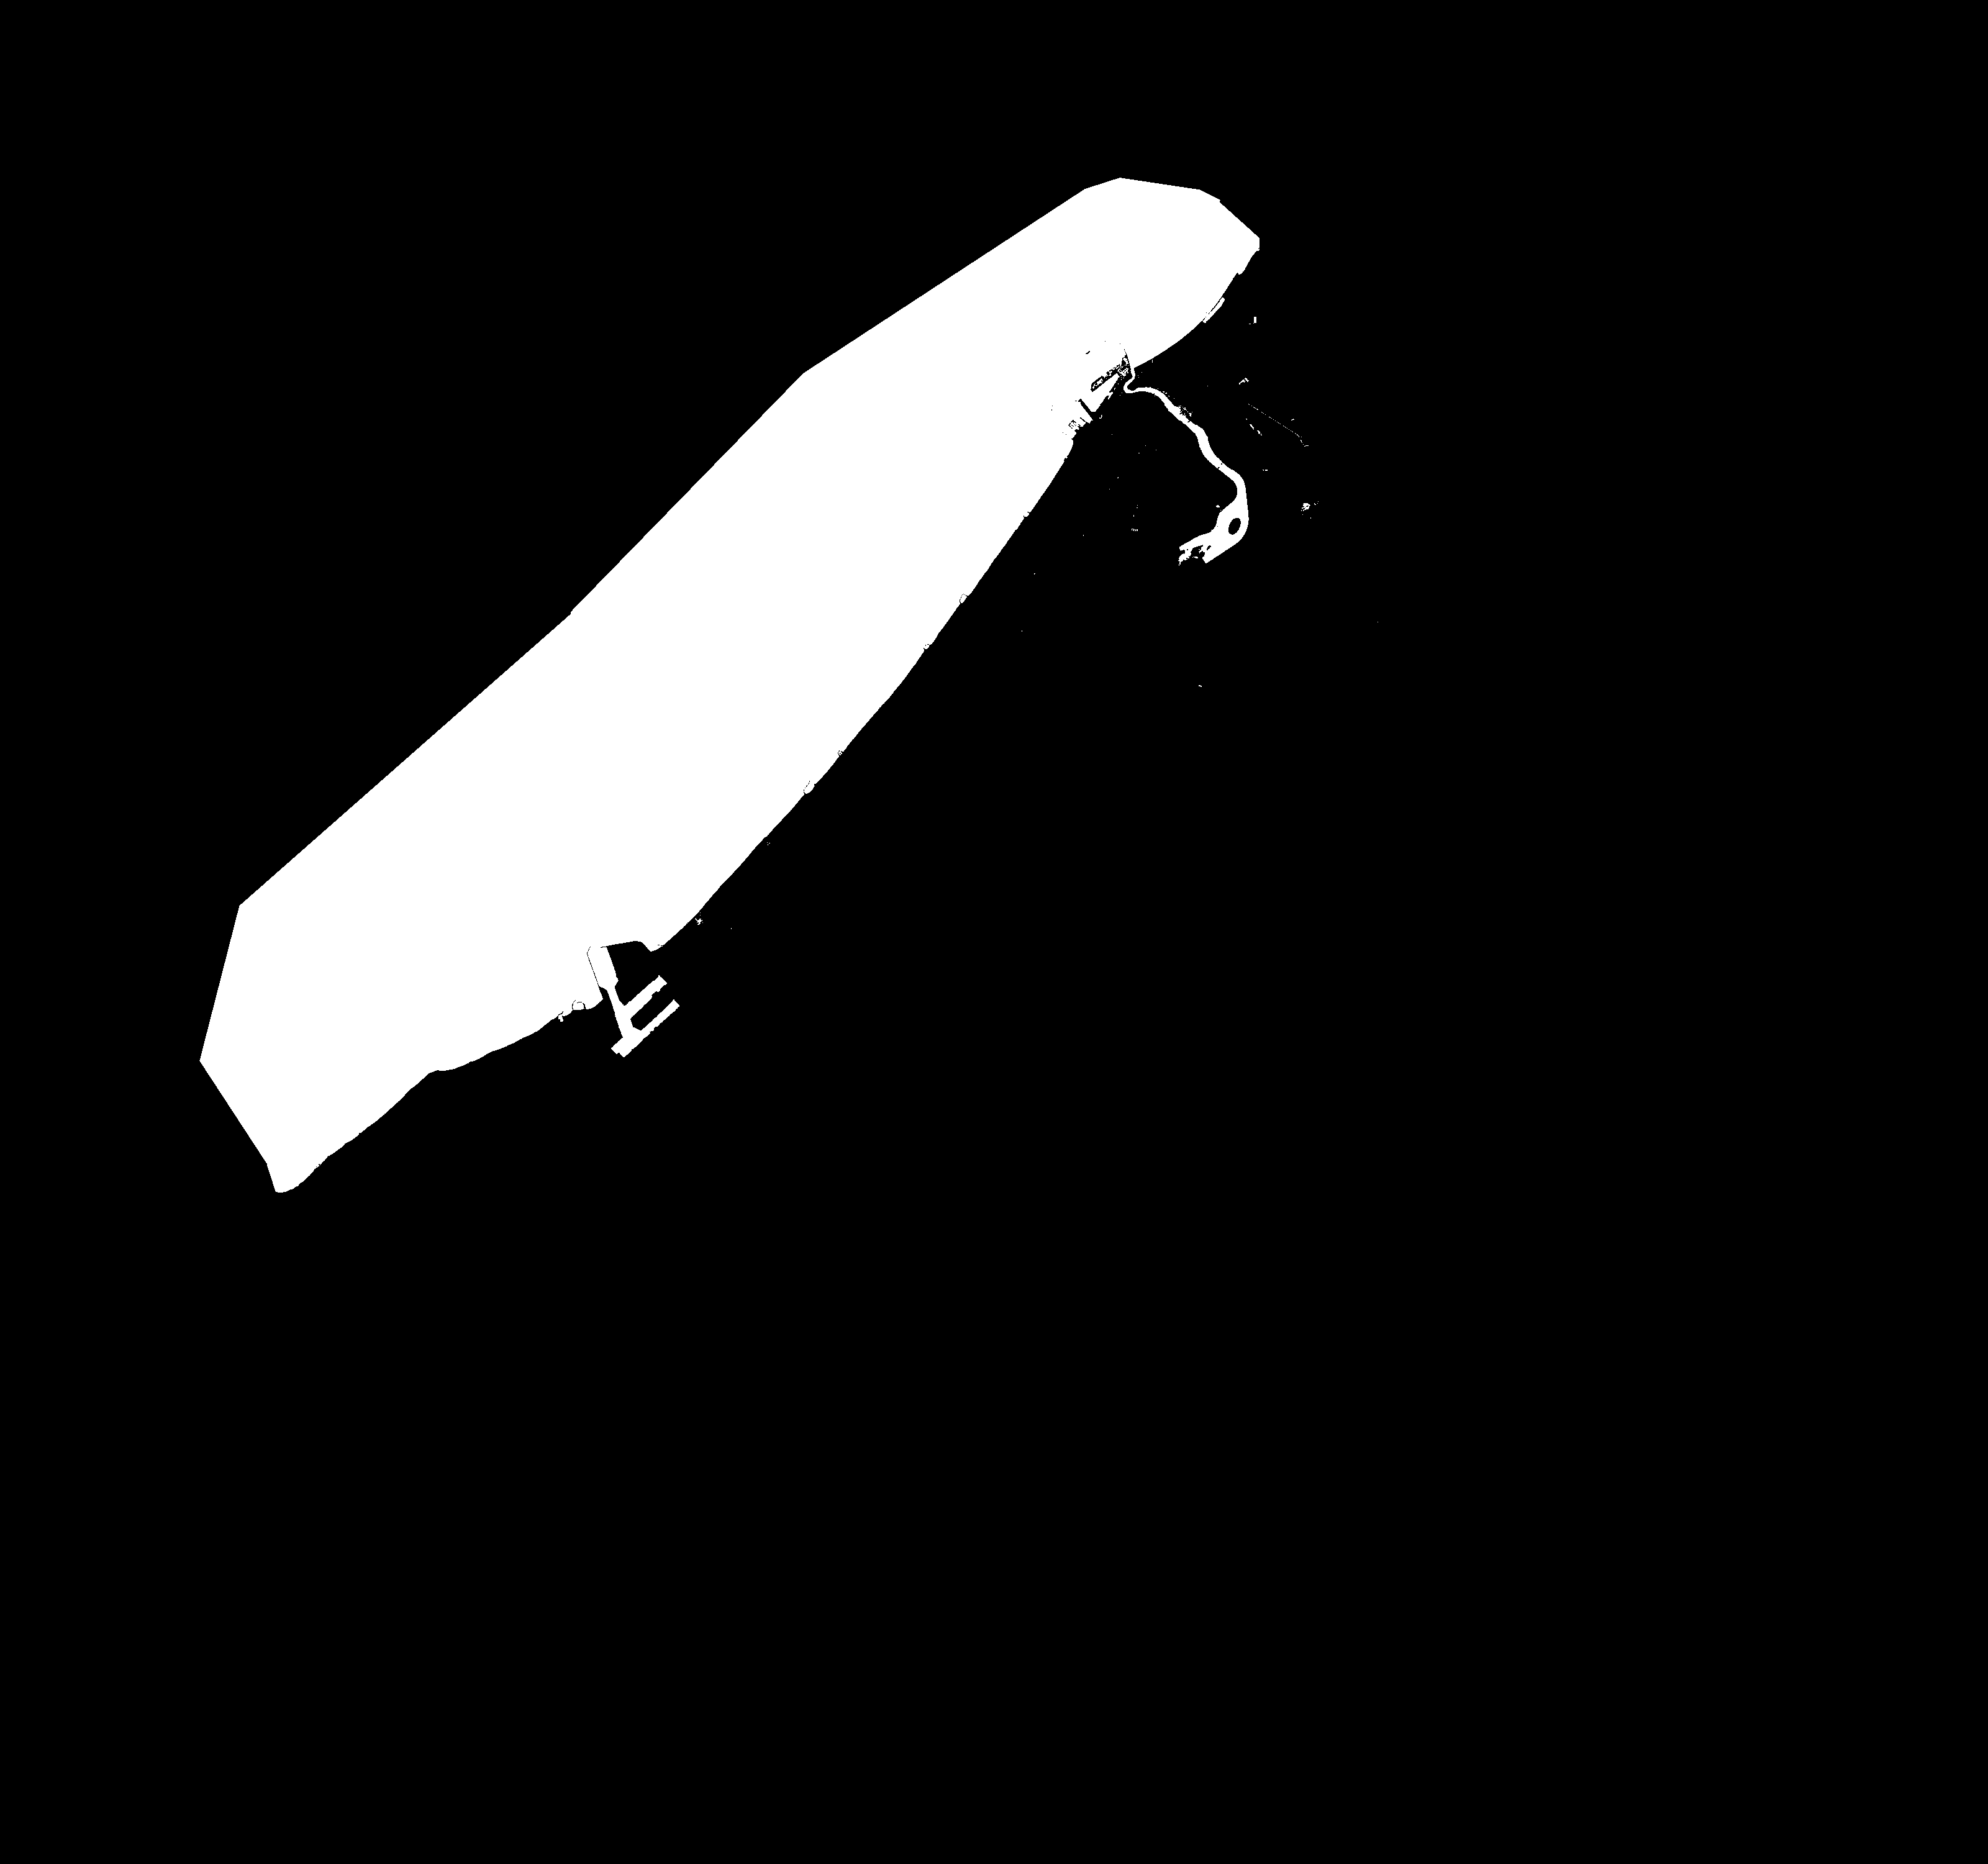
\includegraphics[width=\textwidth-3em]{code/imagedata/analysis/water1984cropped_refd_w}
	\caption{L-5 TM Image (1984) water class}
	\label{fig:water_1984}
\end{minipage}
\end{figure}

The water area could then also be calculated by simply summing the binary image.

\section{Discussion}
After processing the image as explained in the previous chapter, the relative relation inbetween the pictures could be presented with the summed binary image data for both techniques. The result is shown in \cref{fig:analysstreet,fig:analyswater}. \\
One can observe that there are quite high variations in some parts of the water analysis. This is due to failures or insufficient processing, e.g. Image 7 (1990) has a weird cutoff in the northern part, which results in a lower detection of water particles. Unfortunately, the exact reason for this could not be found.\\
Also, the Images taken with LandSat-8 include some streets and other ground areas that are falsely classified as water by the kNN algorithm. A reason for this might be the histogram equalisation. As can be seen in \cref{fig:L8_OLI_16_equalised}, some of the streets appear blue/violet. It is not clear why exactly this happens - since it only occurs on the LandSat-8 data. A cause might be the "sharper" image of the LandSat-8 satellite, due to technology improvements and better satellite stabilisation or the difference between the captured visible spectral bands, since the LandSat-8 OLI has a lower wavelength range compared to the others. This could lead to a different colour profile, and thus an incorrect histogram equalisation.

But also the analysis using the edge detection has some drawbacks.
The edge detection of course detects edges regardless if it's e.g. a border between land and water or a street and water.
\todo[inline]{do this shit!}

However, plotting the trendline in the results (\cref{fig:analysstreet,fig:analyswater}) shows that the initial hypotheses can be confirmed, since the

\todo[inline]{also do this shit!}


Comparing this to officially available demographic data the analysis seems to be qualitatively correct

\todo[inline]{download UN data!}

\begin{figure}[h!]
\centering
\begin{minipage}{.5\textwidth}
	\centering
%	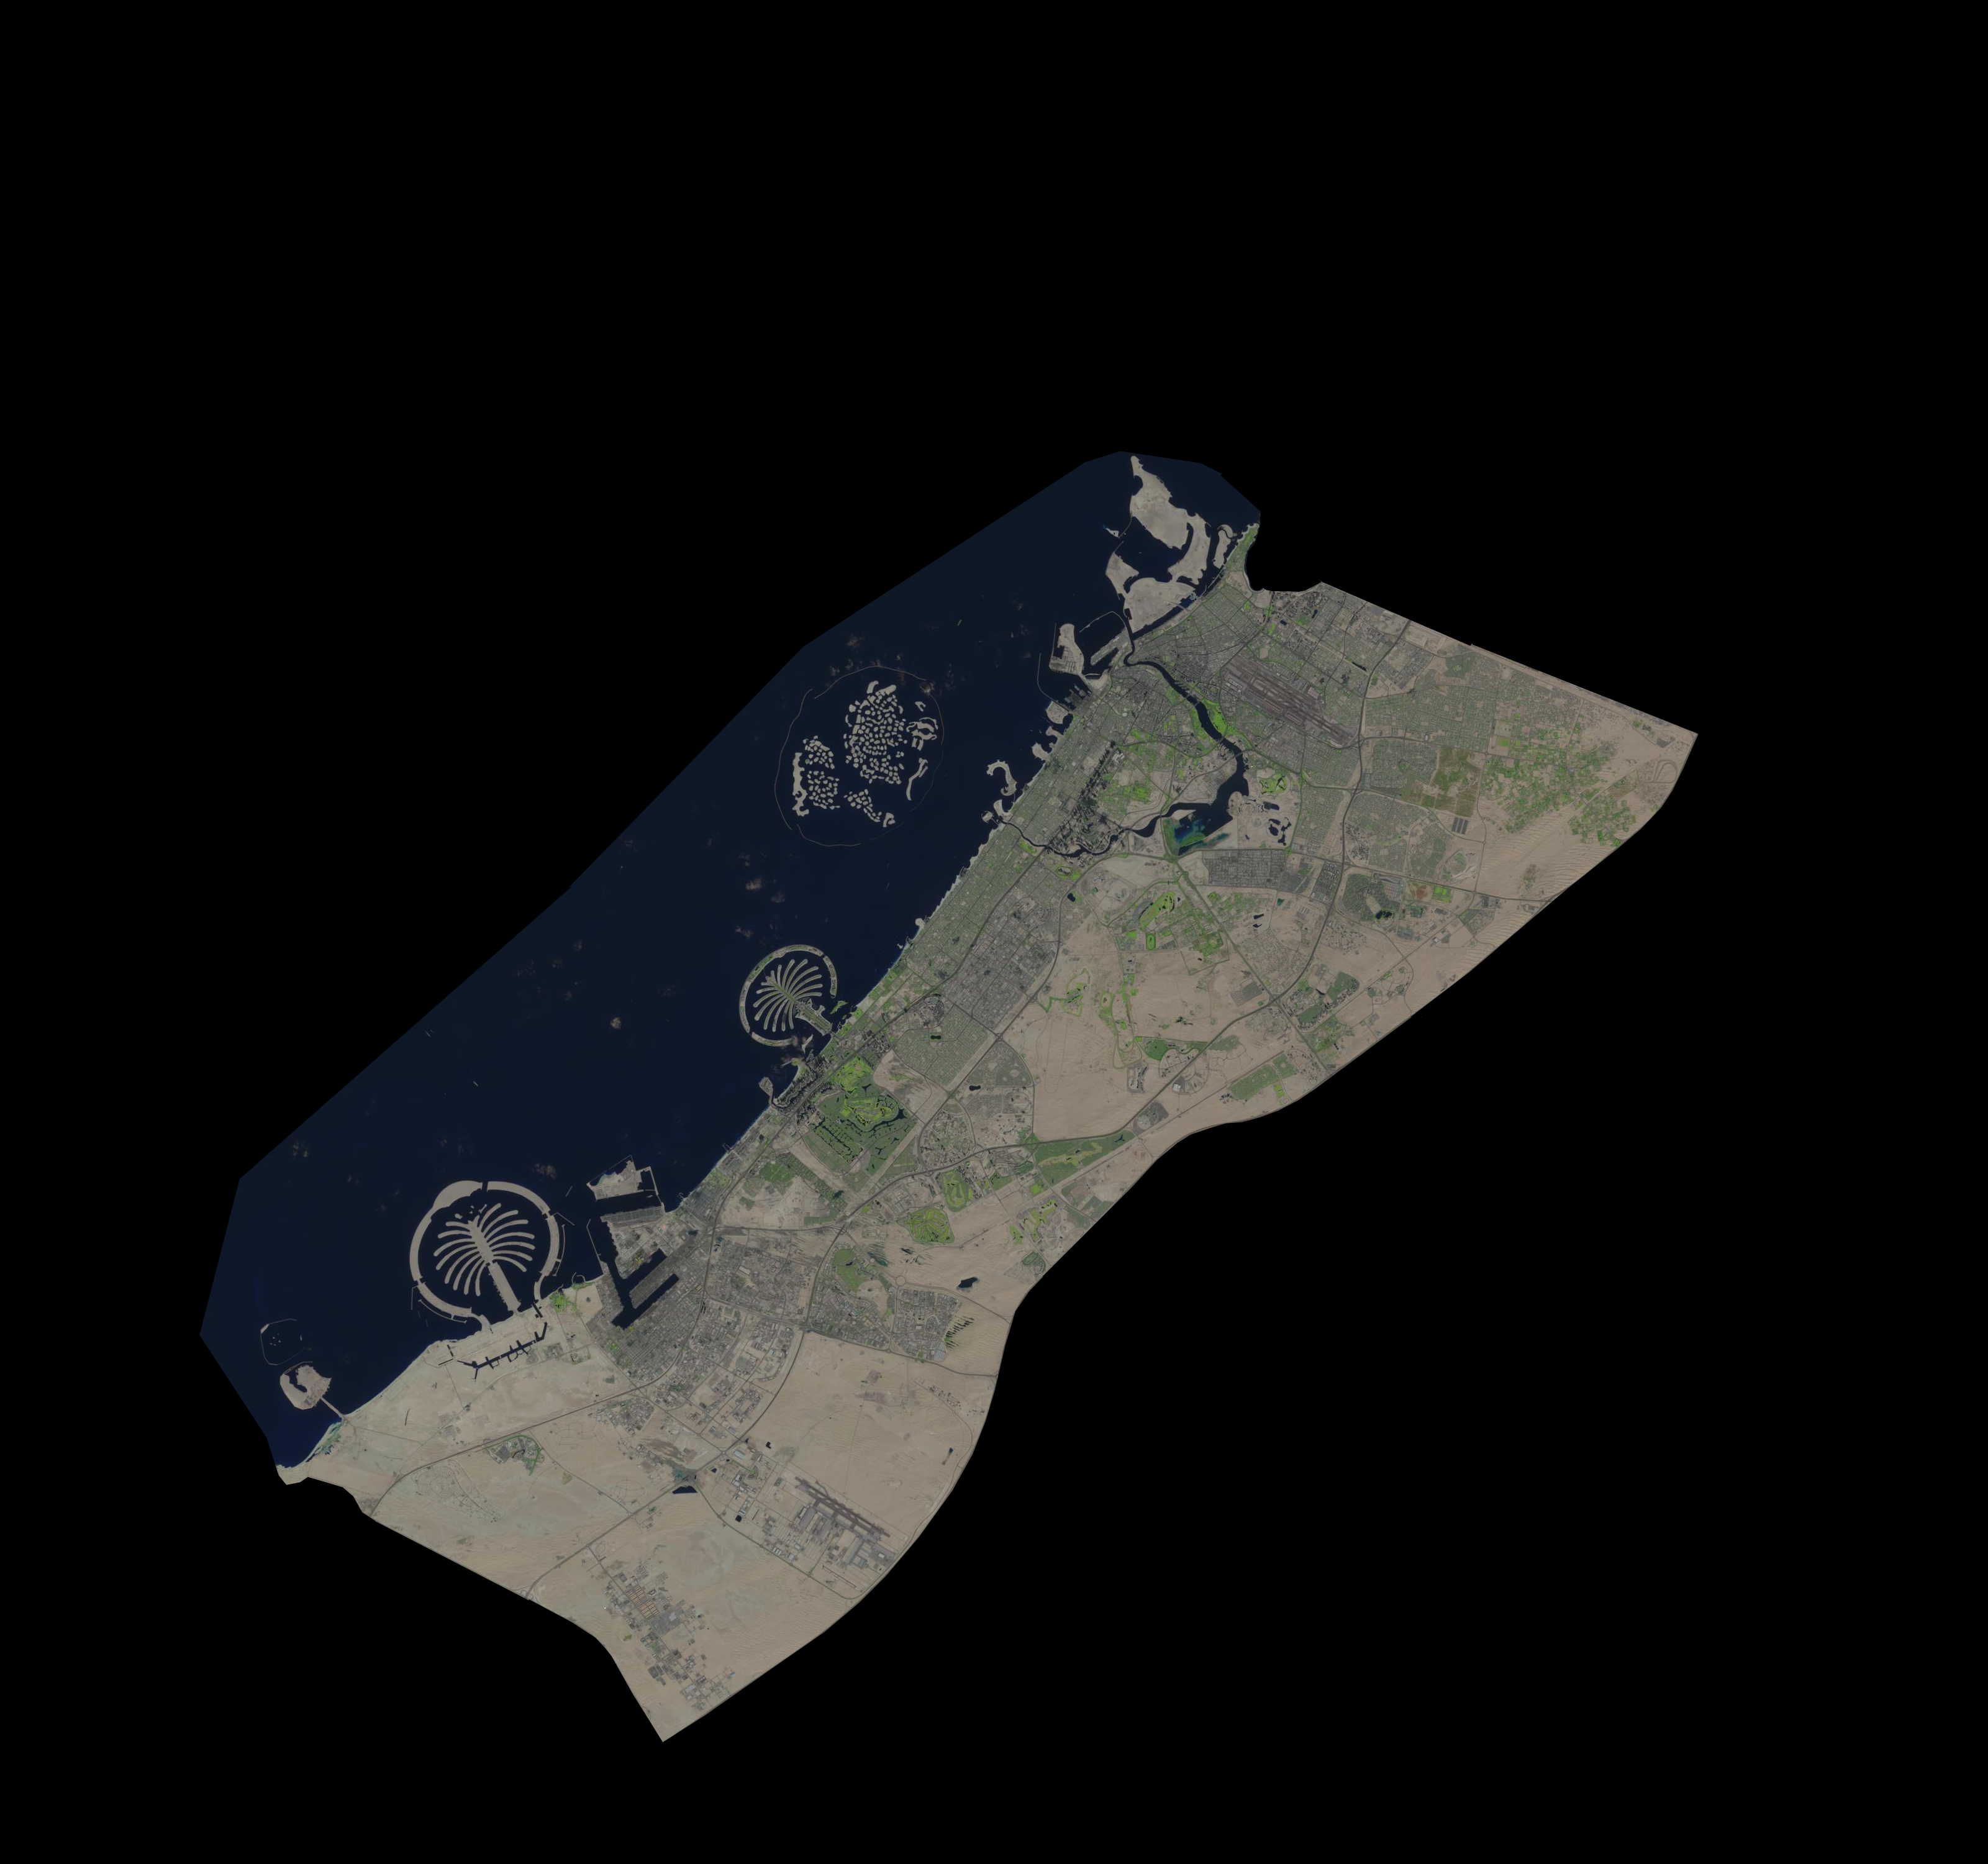
\includegraphics[width=\textwidth-3em]{code/imagedata/alldata/2016cropped}
%	\caption{L-8 OLI Image (2016) cropped}
	\label{fig:analysstreet}
\end{minipage}%
\begin{minipage}{.5\textwidth}
	\centering
%	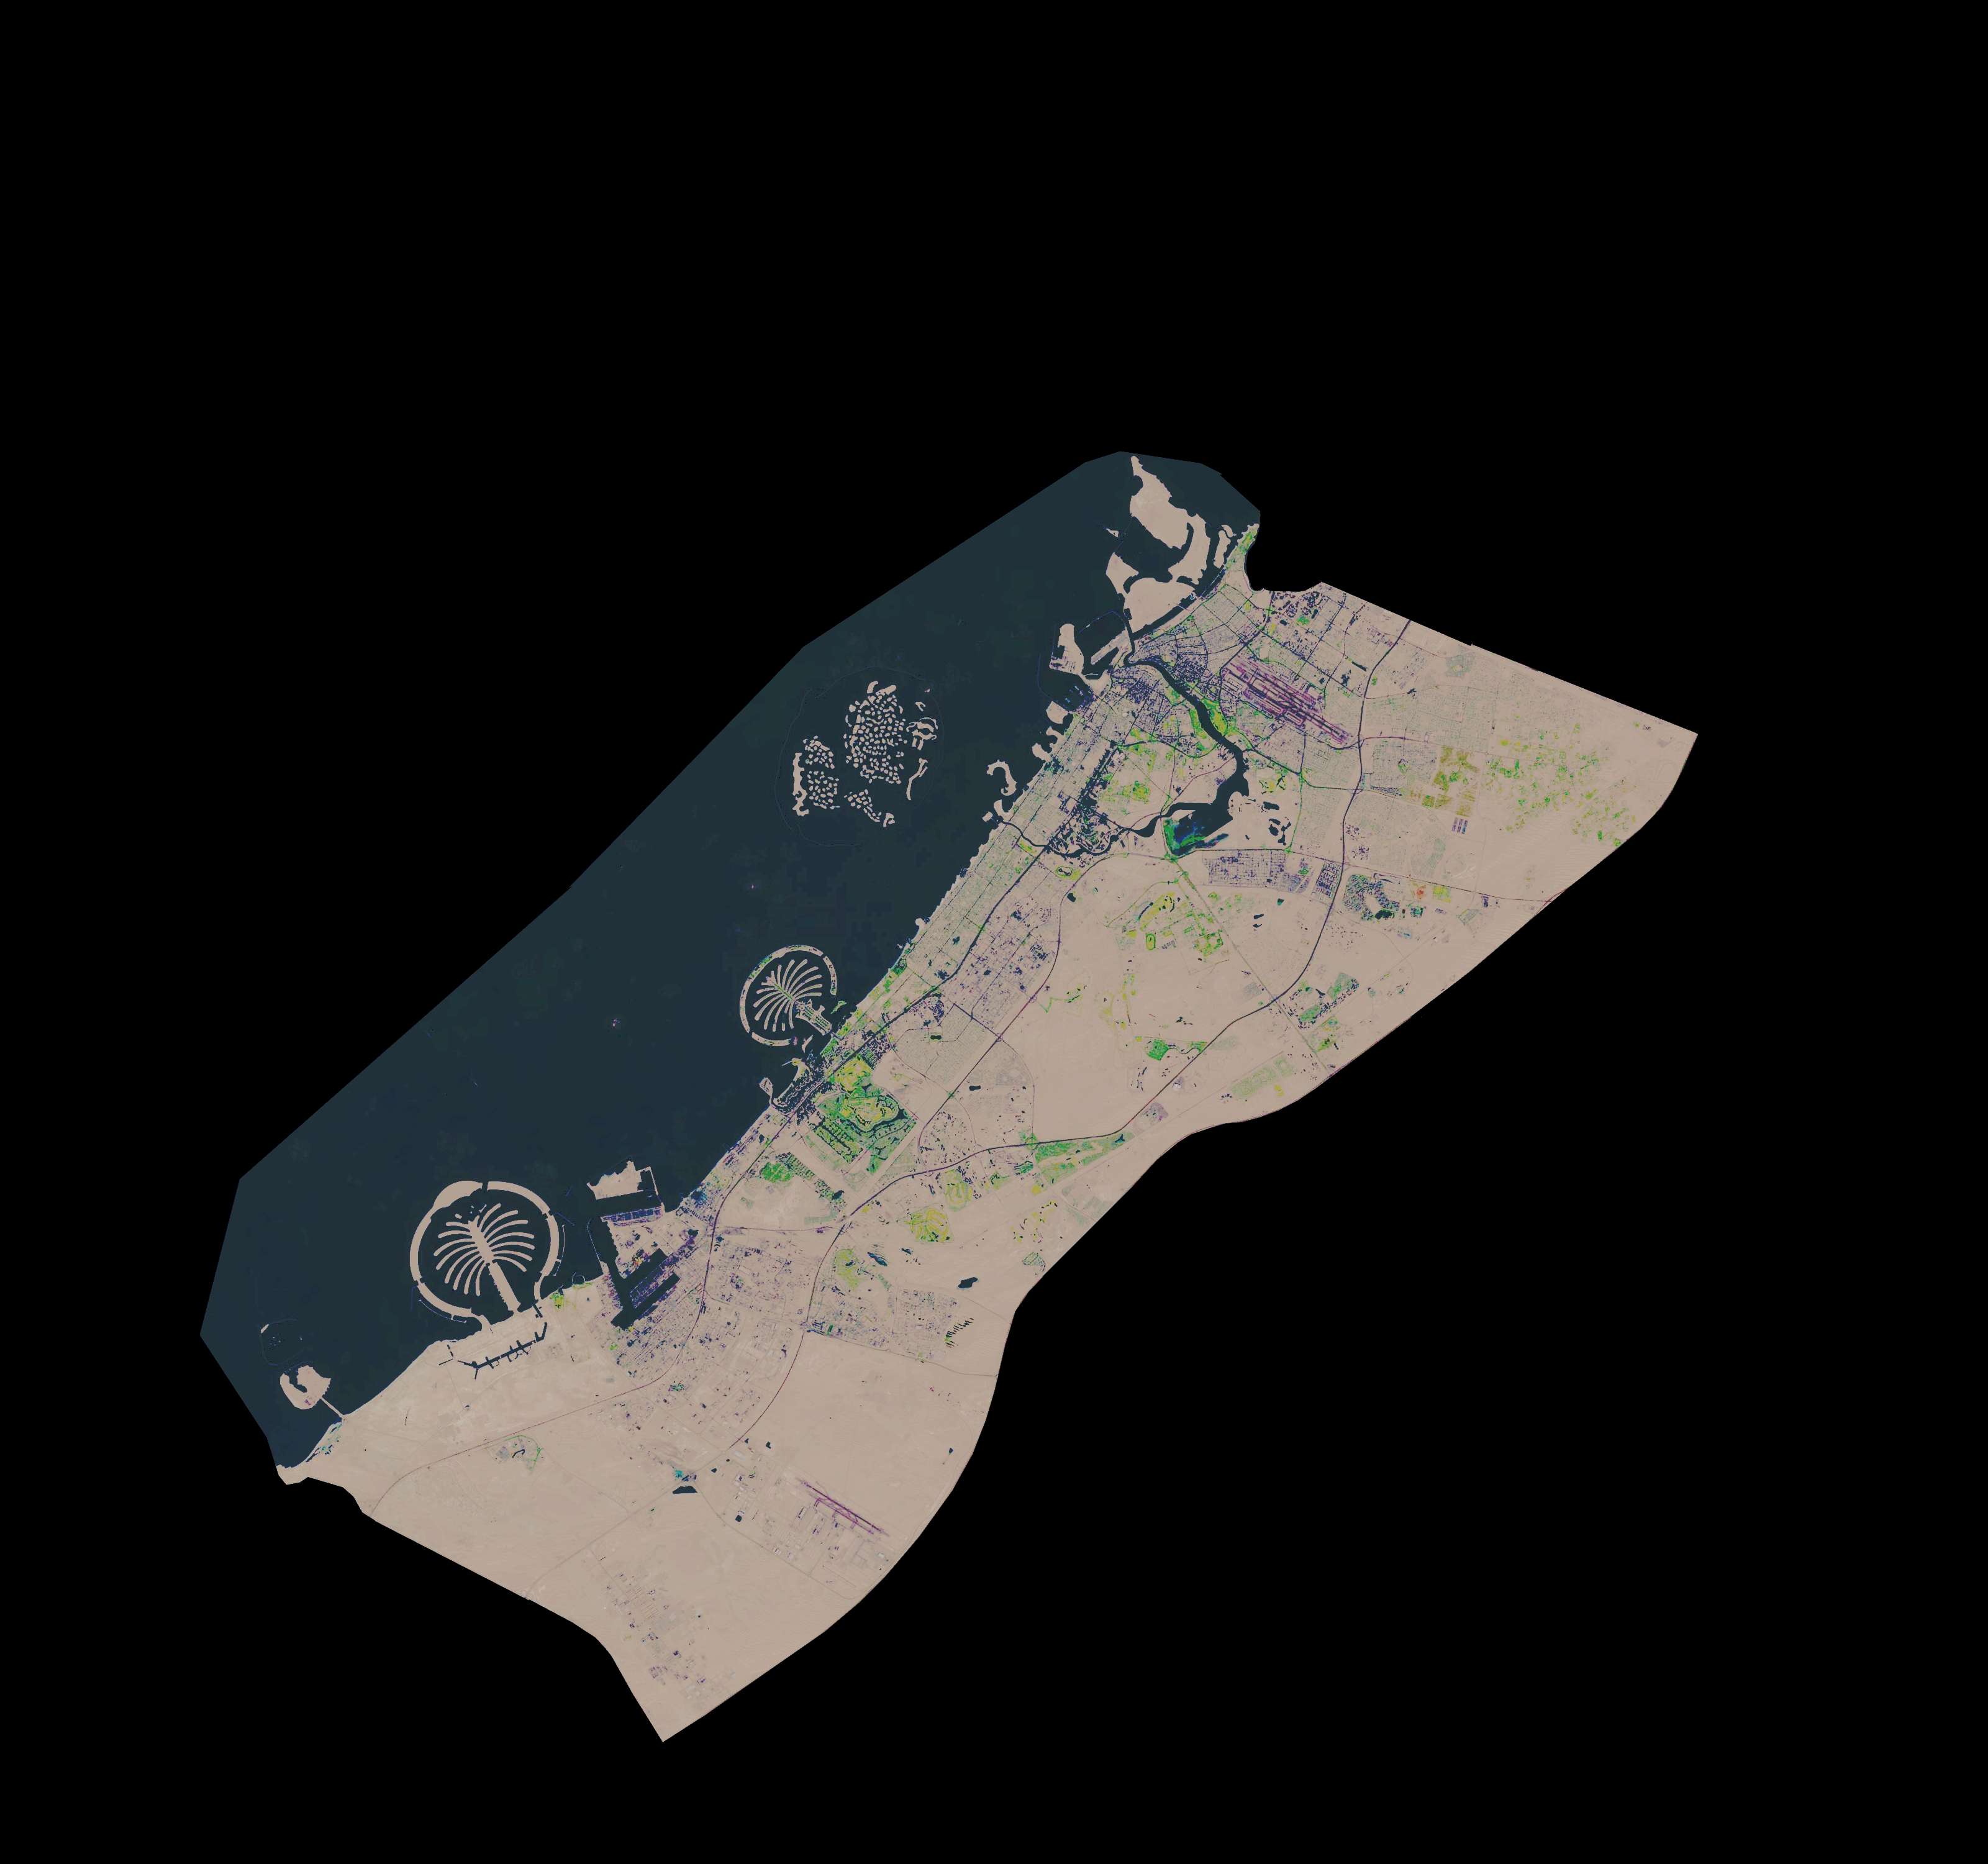
\includegraphics[width=\textwidth-3em]{code/imagedata/alldata/2016cropped_refd}
%	\caption{L-8 OLI Image (2016) cropped and equalized}
	\label{fig:analyswater}
\end{minipage}
\end{figure}



\section{Conclusion}

As stated in the introductory part of this report, Dubai is a very fast growing and expanding city, mainly due to its initially vast oil resources and thus its attraction and accumulation of wealth and wealthy people.\\
This was expected to lead to an increase in infrastructure development, due to the increasing population. Based on these assumptions, two hypotheses were made concerning the expected landscape change in satellite imagery.\\
These hypotheses were examined using LandSat image data starting from the year 1984 until the year 2016. However, due to technical reasons, the limited scope of this report and the unavailability of data for unknown reasons there exist gaps in the data between 2003 to 2008 and 2008 to 2013.\\
Finally, using two different approaches, the hypotheses could be qualitatively verified, thus an observation of Dubai's infrastructure using space-based imagery is feasible and possible with basic algorithmic approaches.

However, since the used algorithmic approach is only basic it could be optimised by a lot, e.g. doing a better classification of water, land and streets and use a better approach for the edge detection than just apply morphological closing to detect the area.\\
Also, in further work one could fill the data gaps with image data provided by other satellites. Another also promising approach would be to use an extended image histogram equalisation, since the spectral bands used to create the data differed throughout the used imagery. Further research should be done to show if there is an approach to account for this issue.\\
For a more accurate result, one could also take into account the classification of vegetation and streets. A quick glance on the data (created during the kNN classification), showed that the vegetation and streets were classified quite accurate in some images. Still, for this report this data was not used, due to limited time and resources.\\
It would also be interesting to create or use an approach that would allow automatic masking and cropping images (which was done manually for this report), for example using overlay-algorithms to detect the best mask fit between two images.

To conclude, the overall approach to observe infrastructure development from space seemed feasible, even on a very basic level, thus it might be interesting to improve this approach by optimising the algorithms and fill the existing gaps in data with more satellite images in further work.































% if appendix needed, uncomment the following lines
The whole Appendix including MATLAB Code, Images and Report-Latex file    can be downloaded from the following githug-repository:

\begin{center}
	\url{https://github.com/art1/UE52-Earth-Observation-Report}{https://github.com/art1/UE52-Earth-Observation-Report}
\end{center}

For the sake of completeness and to ease referencing, the MATLAB Code is also given within this report in the following Appendix A.

\section{MATLAB Code}
\label{Appendix A}

\subsection{ROI Selection and Histogram Equalisation}
\label{selectROI}
\lstinputlisting{code/selectROI.m}

\subsection{Edge Detection}
\label{edgeDetection}
\lstinputlisting{code/proc_edge.m}

\subsection{Colour Analysis}
\label{colouranalysis}
\lstinputlisting{code/proc_water.m}

\section{LandSat Image Data}
\label{Appendix B}
All the used LandSat Image Data can be downloaded using the following identifiers as input for the \textit{Bulk Download Application} provided on the USGS Website

\verbatiminput{code/landsatDataIDs.txt}



% if bibliography needed, uncomment the following lines
\bibliographystyle{plainnat}
\bibliography{biblist}

%%%%%%%%%%%%%%%%% include content end %%%%%%%%%
\end{document}
